\documentclass[11pt, a4paper]{article}

% --- UNIVERSAL PREAMBLE BLOCK ---
\usepackage[a4paper, top=2.5cm, bottom=2.5cm, left=2.5cm, right=2.5cm]{geometry}
\usepackage[utf8]{inputenc}
\usepackage[T1]{fontenc}
\usepackage[english]{babel}

% --- UTILITY PACKAGES ---
\usepackage{amsmath}    % For advanced math environments
\usepackage{booktabs}   % For professional-looking tables
\usepackage{graphicx}   % To include figures
\usepackage{microtype}  % Improves typography and justification
\usepackage{float}      % For improved float control [H]
\usepackage{caption}    % <--- THIS IS THE MISSING LINE
\usepackage{hyperref}   % For clickable links and references (load last)
\usepackage{siunitx}    % For SI units

\hypersetup{
    colorlinks=true,
    linkcolor=blue,
    filecolor=magenta,      
    urlcolor=cyan,
    pdftitle={Bio-Inspired Myriapod Robot Analysis},
    pdfpagemode=FullScreen,
}

% --- DOCUMENT METADATA ---
\title{\textbf{Analysis of a Bio-Inspired Myriapod Robot with a Modified Spine and Legs Linkage}}
\author{Team 01: Varun Karthik \quad Yeshwanth Reddy Gurreddy \quad Jeevan Hebbal Manjunath\\\\\textit{RAS 557: Foldable Robotics}\\ Project Assignment - 2}
\date{\today}

\begin{document}

% --- FRONT MATTER ---
\maketitle

\begin{abstract}
This study investigates the locomotory dynamics of a bio-inspired segmented quadruped robot, designed to analyze the coupling between spinal compliance and leg kinematics. While prior work suggests that compliant spines enhance stability, porting these benefits to meso-scale laminate robots presents significant implementation challenges. We developed a rigid-body MuJoCo simulation which predicted that a stiff, short-spine configuration ($L=50$mm) would minimize lateral oscillations and maximize forward velocity. To validate this, a physical prototype was fabricated using the Smart Composite Microstructures (SCM) process, featuring a \textbf{Parallel Articulation Mechanism (PAM)} spine and four Jansen linkage legs. However, experimental trials revealed a critical simulation-to-reality gap: the physical robot failed to achieve net forward locomotion ($v_x \approx 0$) despite successful kinematic cycling. Analysis attributes this divergence to two primary unmodeled factors: friction cone violations at the cardstock-ground interface and parasitic buckling of the load-bearing laminate links. Rather than validating the spine's efficacy, this study characterizes the dominant structural and frictional barriers that must be overcome before spinal compliance can be effectively exploited in laminate-based quadrupeds.
\end{abstract}
\clearpage
{
    \hypersetup{linkcolor=black}
    \small
    \tableofcontents
}
\thispagestyle{plain}
\clearpage

% =================================================
% 1. INTRODUCTION
% =================================================
\section{Introduction}
\label{sec:introduction}

The development of agile terrestrial robots capable of navigating unstructured environments remains a significant engineering challenge. While traditional wheeled or rigid-body platforms often struggle with terrain irregularities, bio-inspired systems offer a robust alternative by leveraging "morphological intelligence"—the physical encoding of control strategies into the mechanical structure itself. Specifically, arthropods such as myriapods (e.g., \textit{Lithobius forficatus} or stone centipede) utilize segmented body plans coupled with compliant inter-connections to decouple body posture from ground reaction forces. This architecture permits stable locomotion over uneven terrain through passive mechanical adaptation rather than complex active control. 

In this study, we translate these biological principles into a meso-scale, foldable robotic platform using the Smart Composite Microstructures (SCM) manufacturing process. This report details the complete engineering cycle of a segmented, quadrupedal robot designed to investigate the dynamic coupling between spinal compliance and high-order leg kinematics. By utilizing laminate-manufactured foldable robotics, we aim to demonstrate how bio-mimetic compliance can enhance inherent stability in unstructured environments.

\subsection{Motivation and Project Goals}
The primary motivation of this work is to quantify the dynamic trade-offs inherent in compliant segmented locomotion. While hexapedal (6-legged) implementations benefit from inherently stable tripod gaits, they often mask the specific contribution of spinal compliance to stability. By reducing the morphology to a quadruped (4-legged) system, we create a more challenging dynamic environment where the spine's role in maintaining ground contact becomes critical.

Specific engineering goals for this reduced-topology platform include:
\begin{itemize}
    \item \textbf{Synthesize a High-Clearance Morphology:} Integrate single-degree-of-freedom \textbf{Jansen linkages} to generate foot trajectories with superior vertical clearance compared to simple rotary legs.
    \item \textbf{Design a Novel Compliant Spine:} Replace complex multi-stage backbones with a simplified \textbf{Parallel Articulation Mechanism (PAM)} spine, designed to provide tunable lateral flexibility while maintaining torsional rigidity.
    \item \textbf{Bridge Simulation and Reality:} Formulate a physics-based model in MuJoCo to predict the gait dynamics of this quadrupedal system and validate these predictions against a physical SCM prototype.
    \item \textbf{Optimize Passive Dynamics:} Investigate how the stiffness of the X-flexure spine influences the robot's ability to maintain a stable trot gait without complex active feedback.
\end{itemize}

\subsection{Biological and Myriapod Inspiration}
Our design is biologically grounded in the morphology of myriapods. Although we have simplified the system to four legs, we retain the core biological principles that define myriapod locomotion:
\begin{itemize}
    \item \textbf{Segmentation and Articulation:} Myriapods are not rigid beams; they are chains of articulated units. Our two-segment design mimics a single "vertebral" interface of the biological creature, serving as a functional primitive for understanding longer chains.
    \item \textbf{Distributed Propulsion:} Locomotion is driven by the coordinated movement of legs on distinct segments, requiring the spine to mediate forces between the anterior and posterior sections.
    \item \textbf{Passive Adaptation:} The inherent compliance of the exoskeleton allows the body to conform to obstacles passively, reducing the computational burden on the central nervous system.
\end{itemize}

\subsection{From Reference Centipede Microrobot to Our Design}
The direct engineering lineage of this project traces back to the myriapod microrobot architecture established by Hoffman and Wood \cite{Hoffman2011}. Their work successfully demonstrated segmented locomotion using a 3-segment, 6-legged platform. However, to enhance performance and manufacturability at our specific scale, we have introduced \textbf{two} major topological deviations:

\begin{figure}[H]
    \centering
    \fbox{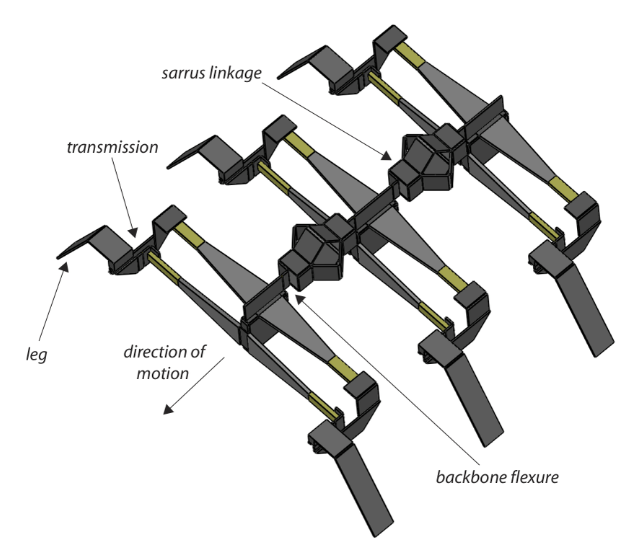
\includegraphics[width=0.35\textwidth]{../figures/Myriapod.png}}
    \caption{The reference myriapod microrobot architecture by Hoffman and Wood \cite{Hoffman2011} which serves as the design inspiration for our segmented morphology. Note the use of sarrus linkages in the spine, which we have evolved into a simplified laminate design.}
    \label{fig:myriapod_reference}
\end{figure}

\begin{enumerate}
    \item \textbf{Morphology Reduction (6 Legs $\rightarrow$ 4 Legs):} We reduced the system from three segments to \textbf{two segments}. This quadrupedal configuration forces the system out of the statically stable "alternating tripod" regime and into a dynamically challenging "trot" regime. By removing the stabilizing support of extra legs, we isolate the spine's active role in stability, making it a critical variable for analysis.
    \item \textbf{Spine Evolution (Sarrus $\rightarrow$ PAM):} The reference robot utilized complex distributed linkages. We replaced this with a discrete \textbf{Parallel Articulation Mechanism (PAM)}. This provides a distinct rotation axis for lateral bending (yaw) while offering high stiffness against vertical bending (pitch) and twisting (roll), preventing the robot from sagging under gravity.
\end{enumerate}

\subsection{Research Objectives and Methodology}
The primary objective of this report is to validate the efficacy of the PAM spine in stabilizing a quadrupedal Jansen-walker. The study is structured as follows:
\begin{itemize}
    \item \textbf{Dynamic Modeling (Section 3):} We formulate a rigid-body physics model in MuJoCo that captures the complex foot locus of the Jansen linkage and the restoring torques of the spine.
    \item \textbf{Parametric Optimization (Section 4):} A sweep is performed to tune the spinal stiffness ($k_{spine}$) to support a stable trot gait.
    \item \textbf{Fabrication \& Characterization (Section 5):} The design is fabricated using laser-machined carbon fiber/cardstock laminates with localized polymer flexures to form the Jansen legs and the spinal interface.
    \item \textbf{Experimental Validation (Section 6):} We compare the forward velocity and lateral oscillation of the prototype against simulation data to quantify the "Sim-to-Real" gap.
\end{itemize}

% =================================================
% 2. ROBOT ARCHITECTURE AND DESIGN
% =================================================
\section{Robot Architecture and Design}
\label{sec:architecture}

The robot morphology is defined by two primary subsystems: the propulsive Jansen legs and the tunable spinal column. Figure~\ref{fig:robot-overview} shows the overall morphology of the robot.

\begin{figure}[H]
    \centering
    % TODO: replace with actual rendered CAD / photograph
    \fbox{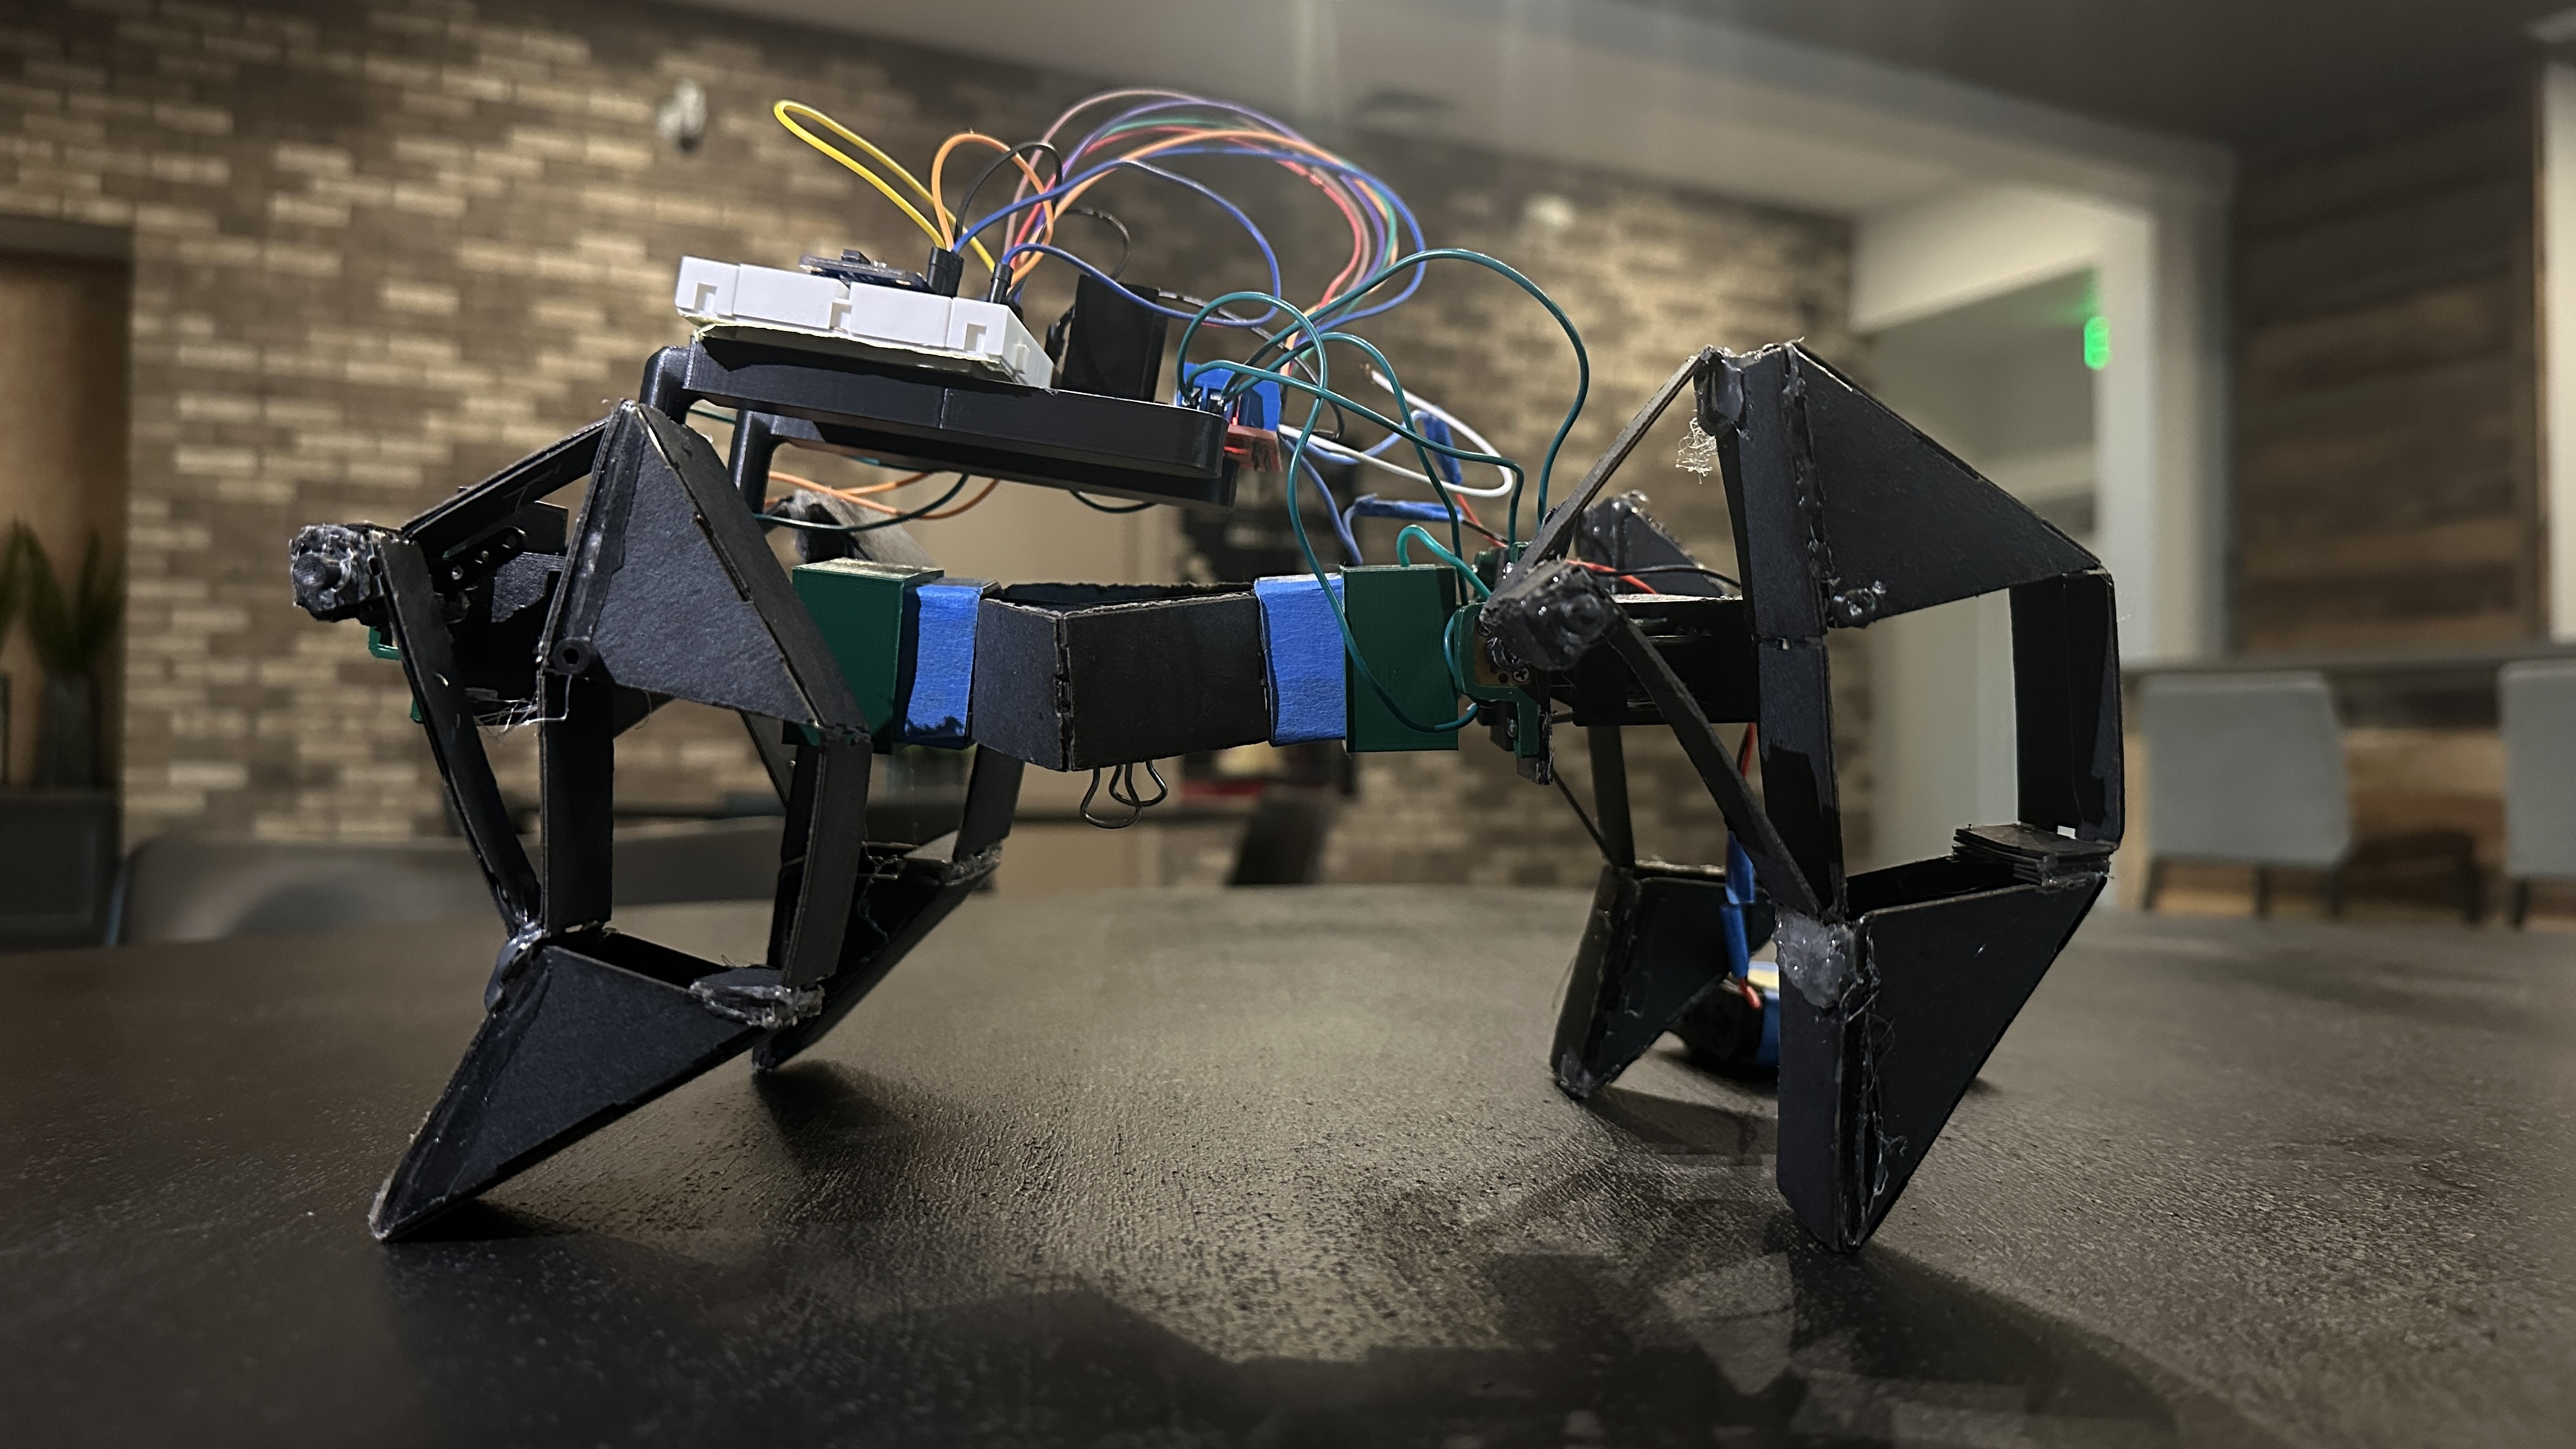
\includegraphics[width=0.5\linewidth]{../figures/my_robot.png}}
    \caption{Overall view of the four-legged myriapod-inspired robot. The Jansen legs are mounted on a central chassis, which is internally connected by a truncated Sarrus-like multi-hinge spine.}
    \label{fig:robot-overview}
\end{figure}

\subsection{Baseline Myriapod Template}
\label{subsec:baseline}
The baseline template follows the myriapod concept: a central body with repeated leg modules and a compliant backbone that couples segment dynamics. In the original work, the backbone is implemented as a sequence of Sarrus linkages and flexures. We retain the overall idea of a compliant backbone linking leg pairs but replace the Sarrus linkage with a simpler \textbf{Parallel Articulation Mechanism (PAM)} spine while also reducing the number of legs and actuators.

\subsection{Jansen Linkage Locomotion}
\label{subsec:jansen}
To achieve ground clearance and a deterministic foot path, we implemented the Jansen linkage. Unlike simple rotary legs, the Jansen mechanism converts rotary input into a complex semi-ovoid trajectory with distinct stance (traction) and swing (lift) phases. The kinematics of the foot position $\mathbf{p}_f$ are a function of the input crank angle $\theta_{crank}$ and the geometric link lengths $\mathbf{l}$:
\begin{equation}
    \mathbf{p}_f(\theta_{crank}) = \mathcal{F}_{Jansen}(\theta_{crank}, \mathbf{l})
\end{equation}
This linkage was selected to mitigate "toe-stubbing"—a common failure mode in low-profile crawlers—by maximizing the vertical lift component of the swing phase. The kinematics and implementation of the Jansen leg are shown in Figure~\ref{fig:jansen-kinematics}.

\begin{figure}[H]
    \centering
    \begin{minipage}[b]{0.45\textwidth}
        \centering
        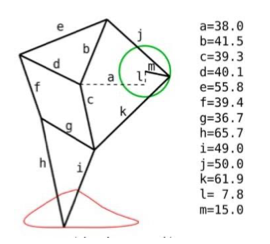
\includegraphics[width=\textwidth]{../figures/jensens_linkage.png}
        \caption*{(a) Idealized Jansen linkage}
    \end{minipage}
    \hfill
    \begin{minipage}[b]{0.45\textwidth}
        \centering
        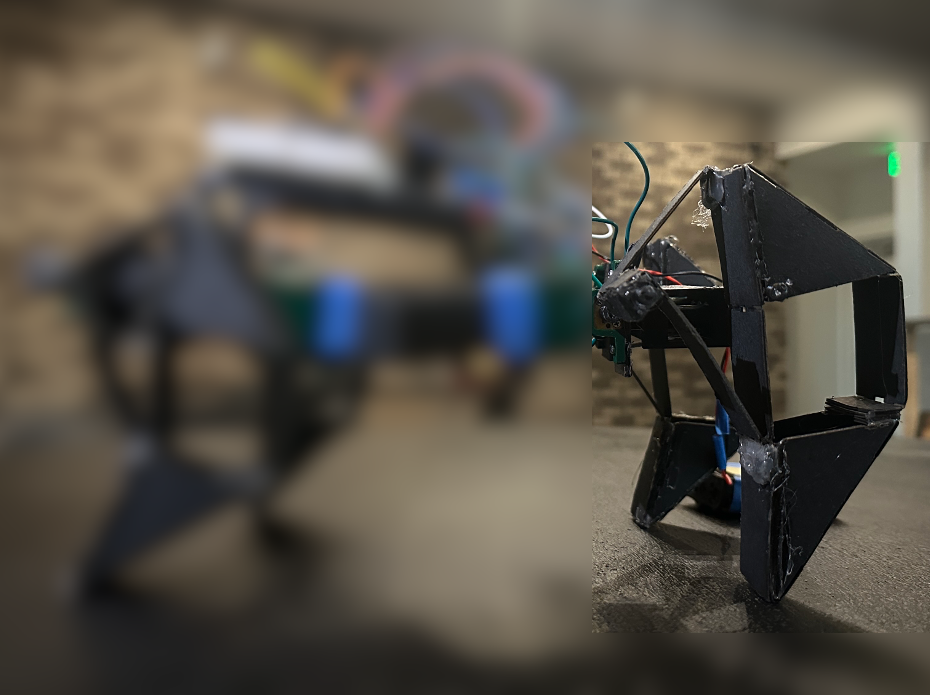
\includegraphics[width=\textwidth]{../figures/my_robot_jensen.png}
        \caption*{(b) Implemented laminate version}
    \end{minipage}
    
    \vspace{0.5cm}
    
    \begin{minipage}[b]{0.45\textwidth}
        \centering
        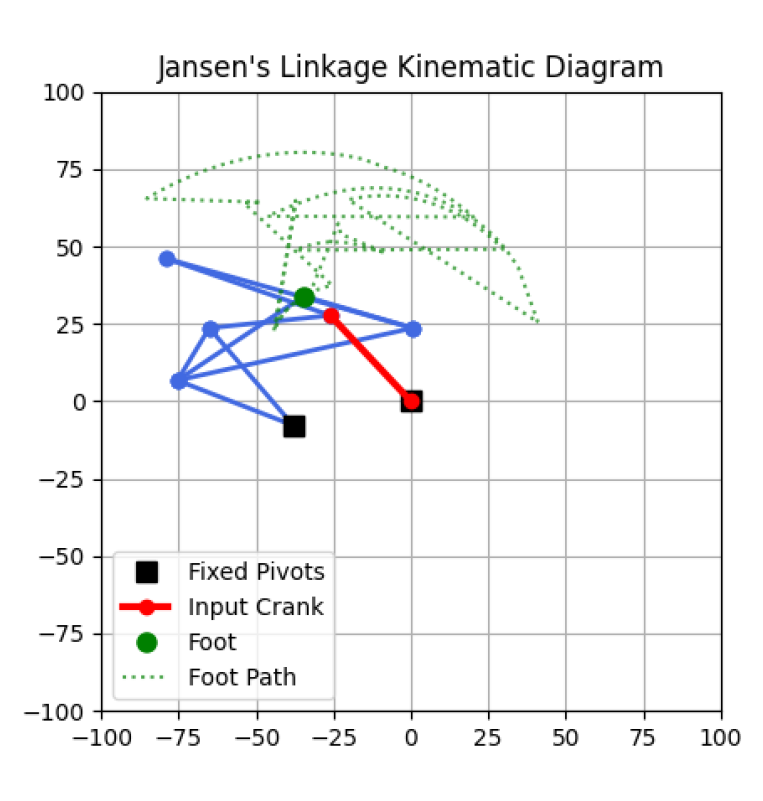
\includegraphics[width=\textwidth]{../figures/jensen_linkage_kinematic_diag.png}
        \caption*{(c) Kinematic analysis}
    \end{minipage}
    \caption{Jansen leg mechanism: (a) Eight-bar linkage schematic driven by a single crank angle $\phi$, producing an ovoid foot trajectory with a flat stance segment. (b) Physical implementation folded into a laminate structure. (c) Kinematic analysis of the Jansen linkage.}
    \label{fig:jansen-kinematics}
\end{figure}

\subsection{Parallel Articulation Mechanism (PAM) Spine}
\label{subsec:spine}
The core innovation of this platform is the variable-geometry spine. Unlike a monolithic flexible beam, our spine is constructed as a discrete linkage (modeled as \texttt{hollow\_wedge} structures in our XML).

\textbf{Variable Stiffness ($k$):} The spine stiffness is governed by the geometry of the flexure hinges and the material properties of the laminate layers. By varying the width of the castellated flexures during the fabrication process, we can tune the torsional spring constant $k_{\theta}$ at the inter-segment joints.
\begin{equation}
    \tau_{restore} = -k_{\theta} (\theta_{yaw}) - c \dot{\theta}_{yaw}
\end{equation}
where $\tau_{restore}$ is the restoring torque helping the robot return to neutral heading after a step cycle.

\textbf{Variable Length ($L$):} The spine design allows for the adjustment of the longitudinal distance between the front and rear hip axes. This parameter, $L$, is critical as it determines the interference potential between the front and rear legs and influences the robot's turning moment of inertia $I_z$:
\begin{equation}
    I_z \approx I_{cm} + m \left(\frac{L}{2}\right)^2
\end{equation}
Optimizing $L$ is a trade-off: a longer spine increases stability (longer wheelbase) but increases the drag moment during turning and may introduce sagging if stiffness is insufficient. The fabricated spine is shown in Figure~\ref{fig:spine}.

\begin{figure}[H]
    \centering
    \begin{minipage}[b]{0.35\textwidth}
        \centering
        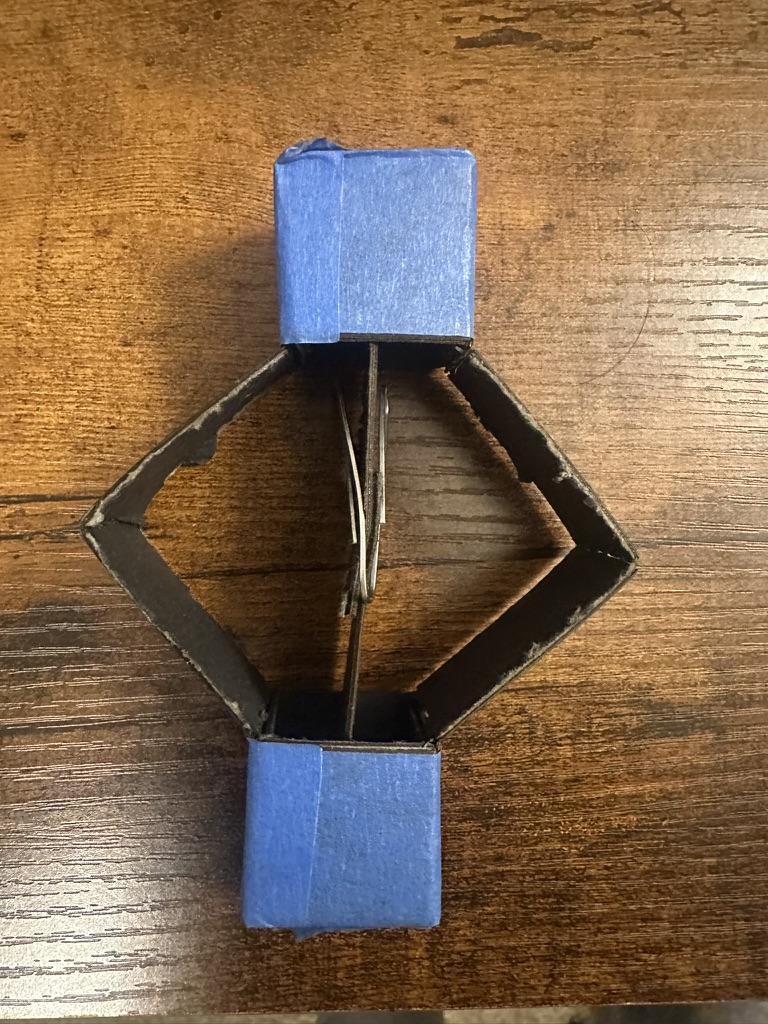
\includegraphics[width=\textwidth]{../figures/spine_design.jpeg}
        \caption*{(a) Fabricated spine mechanism}
    \end{minipage}
    \hfill
    \begin{minipage}[b]{0.35\textwidth}
        \centering
        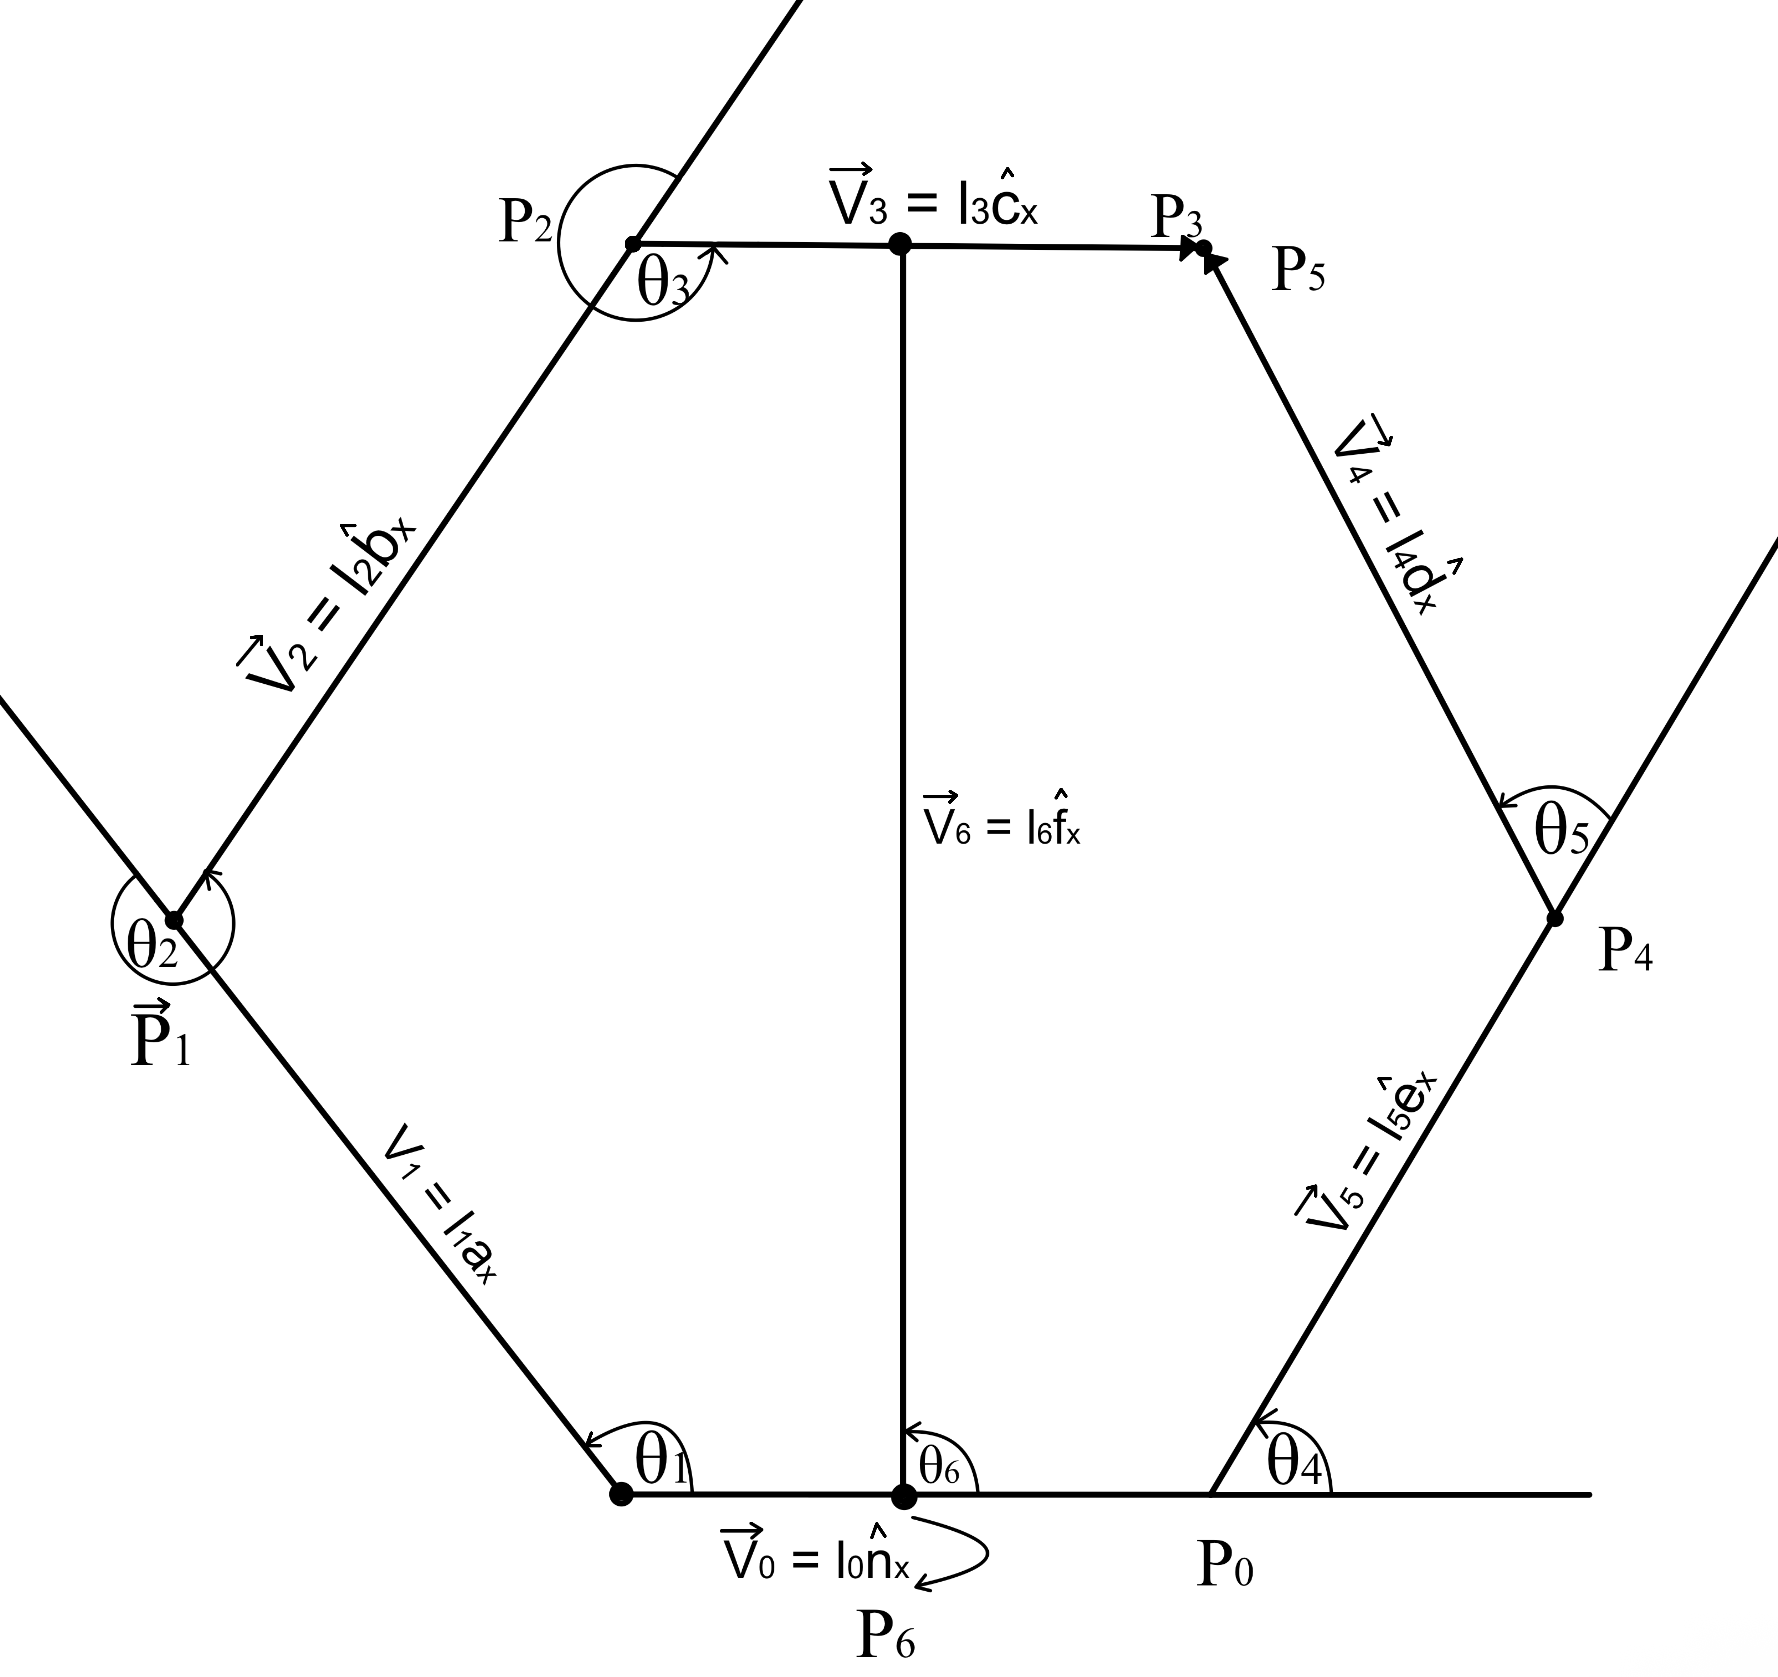
\includegraphics[width=\textwidth]{../figures/spine_kinematic_diag.png}
        \caption*{(b) Kinematic schematic of the spine}
    \end{minipage}
    
    \vspace{0.5cm}
    
    \begin{minipage}[b]{0.4\textwidth}
        \centering
        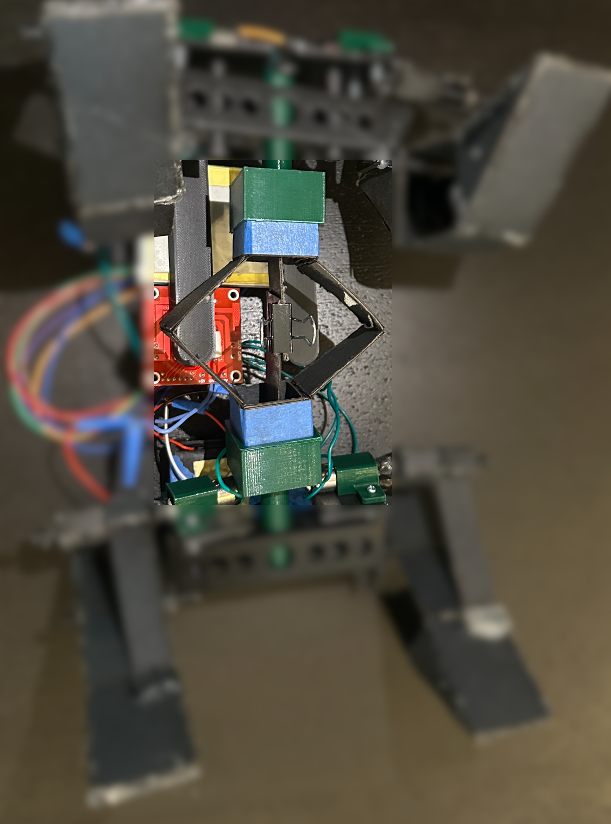
\includegraphics[width=\textwidth]{../figures/my_robot_spine.png}
        \caption*{(c) Fabricated robot with spine installed}
    \end{minipage}
    \caption{The fabricated rigid-link spine mechanism. The length $L$ is adjusted by changing the mounting points of the central wedge segments.}
    \label{fig:spine}
\end{figure}

\subsection{Electronics and Actuation}
The actuation subsystem consists of:
\begin{itemize}
    \item \textbf{Actuators:} 4$\times$ DC motors coupled to the Jansen crank via a transmission gear.
    \item \textbf{Drivers:} 2$\times$ Dual-channel motor drivers (L298N) providing high-current power.
    \item \textbf{Control Unit:} An ESP32 microcontroller generates PWM signals for gait coordination. The ESP32 allows for easy phase adjustments (e.g., switching from trot to pace gaits) via software.
\end{itemize}

% =================================================
% 3. ANALYTICAL KINEMATICS
% =================================================
\section{Analytical Kinematics of the Spine}
\label{sec:analytical_kinematics}

The articulated spine is modeled as a planar three-branch parallel linkage (3R–2R–3R), corresponding to the kinematic diagram in Figure~\ref{fig:spine}b. A Python-based kinematic model was developed to evaluate the workspace and compute Jacobians for force analysis.

\subsection{Variables, Link Vectors, and Points}
All motion is defined in an inertial frame $\mathcal{N}$ with basis $\{\hat{n}_x,\hat{n}_y,\hat{n}_z\}$. The model uses link lengths $l_0,\dots,l_6$ as constants and joint angles $\theta_1,\dots,\theta_6$ as state variables. Planar rotations are represented by the rotation matrix $R_z(\theta)$.

Unit vectors aligned with each link are obtained by rotating the inertial basis:
\begin{align}
    \hat{a}_x &= R_z(\theta_1)\hat{n}_x, & \hat{b}_x &= R_z(\theta_1+\theta_2)\hat{n}_x, \\
    \hat{d}_x &= R_z(\theta_4)\hat{n}_x, & \hat{e}_x &= R_z(\theta_4+\theta_5)\hat{n}_x, \\
    \hat{f}_x &= R_z(\theta_6)\hat{n}_x, & \hat{c}_x &= R_z(\theta_1+\theta_2+\theta_3)\hat{n}_x.
\end{align}

Each rigid link $i$ is defined as a vector $\vec{v}_i = l_i \hat{(\cdot)}_x$. The key joint positions are derived by vector summation:
\begin{align}
    P_0 &= O + \vec{v}_0, & P_6 &= O + \tfrac{1}{2}\vec{v}_0, \\
    P_3 &= O + \vec{v}_1 + \vec{v}_2 + \vec{v}_3, & P_5 &= P_0 + \vec{v}_4 + \vec{v}_5, \\
    P_7 &= P_6 + \vec{v}_6.
\end{align}
Points $P_0$ and $P_6$ lie on the rear chassis, while $P_3$, $P_5$, and $P_7$ lie on the moving front chassis.

\subsection{Loop-Closure Constraints}
For a valid configuration, the branches must meet at the front chassis, and the central spine strut must connect to the chassis center. The following loop-closure constraints are enforced:
\begin{align}
    \mathbf{c}_1 &= P_3 - P_5 = \mathbf{0}, \\
    \mathbf{c}_2 &= P_5 - P_7 - \tfrac{1}{2}\vec{v}_3 = \mathbf{0}.
\end{align}
These constraints ensure the front and rear platforms remain connected via the parallel branches while allowing the spine to bend.

\subsection{Jacobian and Force/Velocity Mapping}
To map actuator torques to endpoint forces, we differentiate the position of the spine tip $P_7$ with respect to the actuated joints $\boldsymbol{\theta}_a = [\theta_4, \theta_5, \theta_6]^T$. The planar Jacobian is:
\begin{equation}
    J(\boldsymbol{\theta}) = \frac{\partial}{\partial\boldsymbol{\theta}_a} \begin{bmatrix} x_7(\boldsymbol{\theta}) \\ y_7(\boldsymbol{\theta}) \end{bmatrix}
\end{equation}
This Jacobian enables two critical analyses:
\begin{itemize}
    \item \textbf{Force Mapping:} A planar force $\mathbf{F}_{\text{ee}}$ applied at $P_7$ generates joint torques $\boldsymbol{\tau}_a = J^{\mathsf{T}} \mathbf{F}_{\text{ee}}$. For a peak vertical load of $F_y \approx \SI{4}{N}$, the model predicts joint torques of approximately \SI{1}{N\,m}, validating the flexure stiffness design.
    \item \textbf{Velocity Mapping:} The front chassis velocity is related to joint rates by $\dot{P}_7 = J(\boldsymbol{\theta}) \dot{\boldsymbol{\theta}}_a$.
\end{itemize}


% =================================================
% 3. MUJOCO DYNAMIC MODELING
% =================================================
\section{MuJoCo Dynamic Model} \label{sec:mujoco-model}

We use MuJoCo as the primary environment for dynamic simulation. The model captures rigid-body dynamics, joint constraints, contact physics, and the electromechanical behavior of the actuators. The final model is generated procedurally using a Python builder (`model\_builder.py`) to ensure the kinematic tree matches the CAD layout of the physical prototype.

\subsection{Code Repository}
\label{subsec:code-repository}
The complete MuJoCo model, simulation scripts, and post-processing code are available in our public GitHub repository:
\begin{center}
\url{https://github.com/RAS557-Jansen-Spine/Robot/tree/mujoco-simulation}
\end{center}
This repository includes:
\begin{itemize}
    \item The procedural model builder (\texttt{model\_builder.py})
    \item Complete XML model definitions
    \item Simulation control scripts
    \item Data analysis and plotting utilities
\end{itemize}

\subsection{Model Organization} \label{subsec:model-organization}
The kinematic tree is structured to replicate the physical assembly:
\begin{itemize}
    \item \textbf{Worldbody:} Contains a planar floor with tangential friction ($\mu=0.5$).
    \item \textbf{Chassis:} A free-floating root body (`chassis`) representing the upper and lower decks. It serves as the attachment point for the front legs and the spine.
    \item \textbf{Spine Subtree:} A chain of bodies (`inner\_segment`, `inner\_shaft`) connected by hinge joints. These joints model the compliant flexures of the physical spine.
    \item \textbf{Leg Subassemblies:} Four independent leg structures. Each leg is a closed-loop kinematic chain. To model this in MuJoCo's tree structure, the loops are broken and re-connected using equality constraints.
\end{itemize}

\subsection{Link Geometry and Mass Properties}
To ensure kinematic equivalence between the simulation and the physical prototype, the dimensions of every link in the Jansen mechanism were directly exported from the CAD design used for manufacturing. Table~\ref{tab:link-props} details the specific body parameters.

\begin{table}[H]
    \centering
    \caption{Geometric and Inertial Properties of Robot Links}
    \label{tab:link-props}
    \begin{tabular}{llccc}
        \toprule
        \textbf{Link Name} & \textbf{Geom Type} & \textbf{Dimensions (L $\times$ W $\times$ H) [mm]} & \textbf{Density [$kg/m^3$]} & \textbf{Mass [g]} \\
        \midrule
        \texttt{Chassis} & Box & $150 \times 25 \times 30$ & 1000 & $\approx 10$ \\
        \texttt{Link\_0} (Crank) & Box & $39.4 \times 30 \times 1.0$ & 1000 & $\approx 1.2$ \\
        \texttt{Link\_1} & Box & $39.4 \times 30 \times 1.0$ & 1000 (override: 10) & $\approx 1.2$ \\
        \texttt{Link\_2} & Box & $2.0 \times 30 \times 1.0$ & 1000 & $<0.1$ \\
        \texttt{Link\_3} & Box & $50.0 \times 15 \times 1.0$ & 1000 & $\approx 0.75$ \\
        \texttt{Link\_5} & Box & $61.9 \times 15 \times 1.0$ & 1000 & $\approx 0.93$ \\
        \texttt{Wedge\_Face} & Mesh & Defined by `tri\_face` vertices & 1000 & Variable \\
        \bottomrule
    \end{tabular}
\end{table}

\textbf{Justification of Values:}
\begin{itemize}
    \item \textbf{Dimensions:} The lengths of links 0, 1, 3, and 5 correspond to the specific Jansen linkage ratios required to produce the desired ovoid foot trajectory. Any deviation here would distort the step height and stride length.
    \item \textbf{Thickness:} All links share a thickness of 1.0mm (modeled as `0.0005` half-extents), which matches the 5-layer laminate stack (Rigid-Adhesive-Flex-Adhesive-Rigid) used in SCM.
    \item \textbf{Density:} A uniform density of $1000~kg/m^3$ was chosen to approximate the composite density of the cardstock ($\approx 800~kg/m^3$), adhesive, and felxure layers. This simplifies the inertial calculation while remaining physically plausible.
    \item \textbf{Triangular Geometry:} The wedge components use mesh geometries (`tri\_face\_1`, `tri\_face\_2`) rather than simple boxes because the triangular shape is functionally critical for the Jansen mechanism's node connections.
\end{itemize}

\subsection{Actuator and Motor Modeling}
\label{subsec:motor-modeling}
The physical robot is actuated by four Pololu DC gearmotors driven by L298N motor drivers. Due to the high gear reduction of these motors, the system dynamics are dominated by internal damping and back-EMF, resulting in a steady-state angular velocity that is roughly proportional to the applied voltage.

To model this behavior in MuJoCo without implementing a complex electrical subsystem, we approximate the gearmotor and driver assembly as a \texttt{velocity} actuator. Unlike a raw DC motor model where control input corresponds to torque, the \texttt{velocity} actuator accepts a target angular velocity ($\omega_{ref}$) as the control signal. The force generation is governed by a proportional gain:
\begin{equation}
    F = k_{gain} (\omega_{ref} - \omega_{act})
\end{equation}
where $F$ is the applied force, $\omega_{act}$ is the current joint velocity, and $k_{gain}$ acts as a stiffness term. We empirically tuned this gain to $k_v = 5.0$ so that the simulated joint accelerations matched the observed hardware spin-up characteristics of the Pololu motors. The control range was limited to $\pm 20$ rad/s to match the maximum speed observed at the nominal 5V operating voltage.

\textbf{Actuator Definition:}
\begin{verbatim}
<actuator>
  <velocity name="motor_joint_1_vel" joint="motor_joint_1" 
            kv="5.0" ctrlrange="-20 20"/>
  ...
</actuator>
\end{verbatim}
The `ctrlrange` limits the maximum angular velocity to $\pm 20$ rad/s, consistent with the 5V supply voltage used in our experiments.

\subsection{Simulation Parameters}
\label{subsec:sim-params}
Key simulation parameters were chosen to balance numerical stability with physical realism. Table~\ref{tab:mujoco-params} summarizes these values and provides the physical justification for each choice.

\begin{table}[H]
    \centering
    \caption{Key MuJoCo Simulation Parameters and Physical Justification}
    \label{tab:mujoco-params}
    \begin{tabular}{p{0.25\textwidth} p{0.25\textwidth} p{0.4\textwidth}}
        \toprule
        \textbf{Parameter} & \textbf{Value} & \textbf{Physical/Numerical Justification} \\
        \midrule
        \textbf{Timestep} & 0.001 s & Selected to capture high-frequency contact dynamics while maintaining stable RK4 integration. A larger step (e.g., 0.01s) would cause instability in the stiff flexure joints. \\
        \midrule
        \textbf{Integrator} & RK4 (Runge-Kutta 4) & Provides higher-order accuracy for orbital stability compared to Euler, critical for simulating periodic gaits without energy drift. \\
        \midrule
        \textbf{Gravity} & $(0, 0, -9.81) \, m/s^2$ & Standard Earth gravity, aligned with the vertical Z-axis of the world frame. \\
        \midrule
        \textbf{Joint Damping} & 0.1 Nms/rad & Models the inherent energy dissipation of the flexures and air resistance. Without this, the un-damped flexures would oscillate indefinitely, unlike the real robot. \\
        \midrule
        \textbf{Joint Armature} & 0.01 $kg \cdot m^2$ & Adds a small "virtual inertia" to the joints. This is a numerical trick to improve stability for very light links (like the cardstock legs) by preventing infinite accelerations from constraint forces. \\
        \midrule
        \textbf{Geom Density} & 1000 $kg/m^3$ & Approximates the composite density of the cardstock/flexure/adhesive laminate used in SCM fabrication (similar to water or dense plastic). \\
        \midrule
        \textbf{Friction} & 0.5 0.1 0.1 & Anisotropic Coulomb friction. The high tangential friction (0.5) provides forward traction for the feet, while low torsional/rolling friction (0.1) allows for necessary slip during turning maneuvers. \\
        \midrule
        \textbf{Actuator Gain ($k_v$)} & 5.0 & Empirical stiffness gain for the velocity actuator. This value was tuned to approximate the transient response of the Pololu gearmotors under load. \\
        \bottomrule
    \end{tabular}
\end{table}

\begin{figure}[H]
    \centering
    \begin{minipage}[b]{0.48\textwidth}
        \centering
        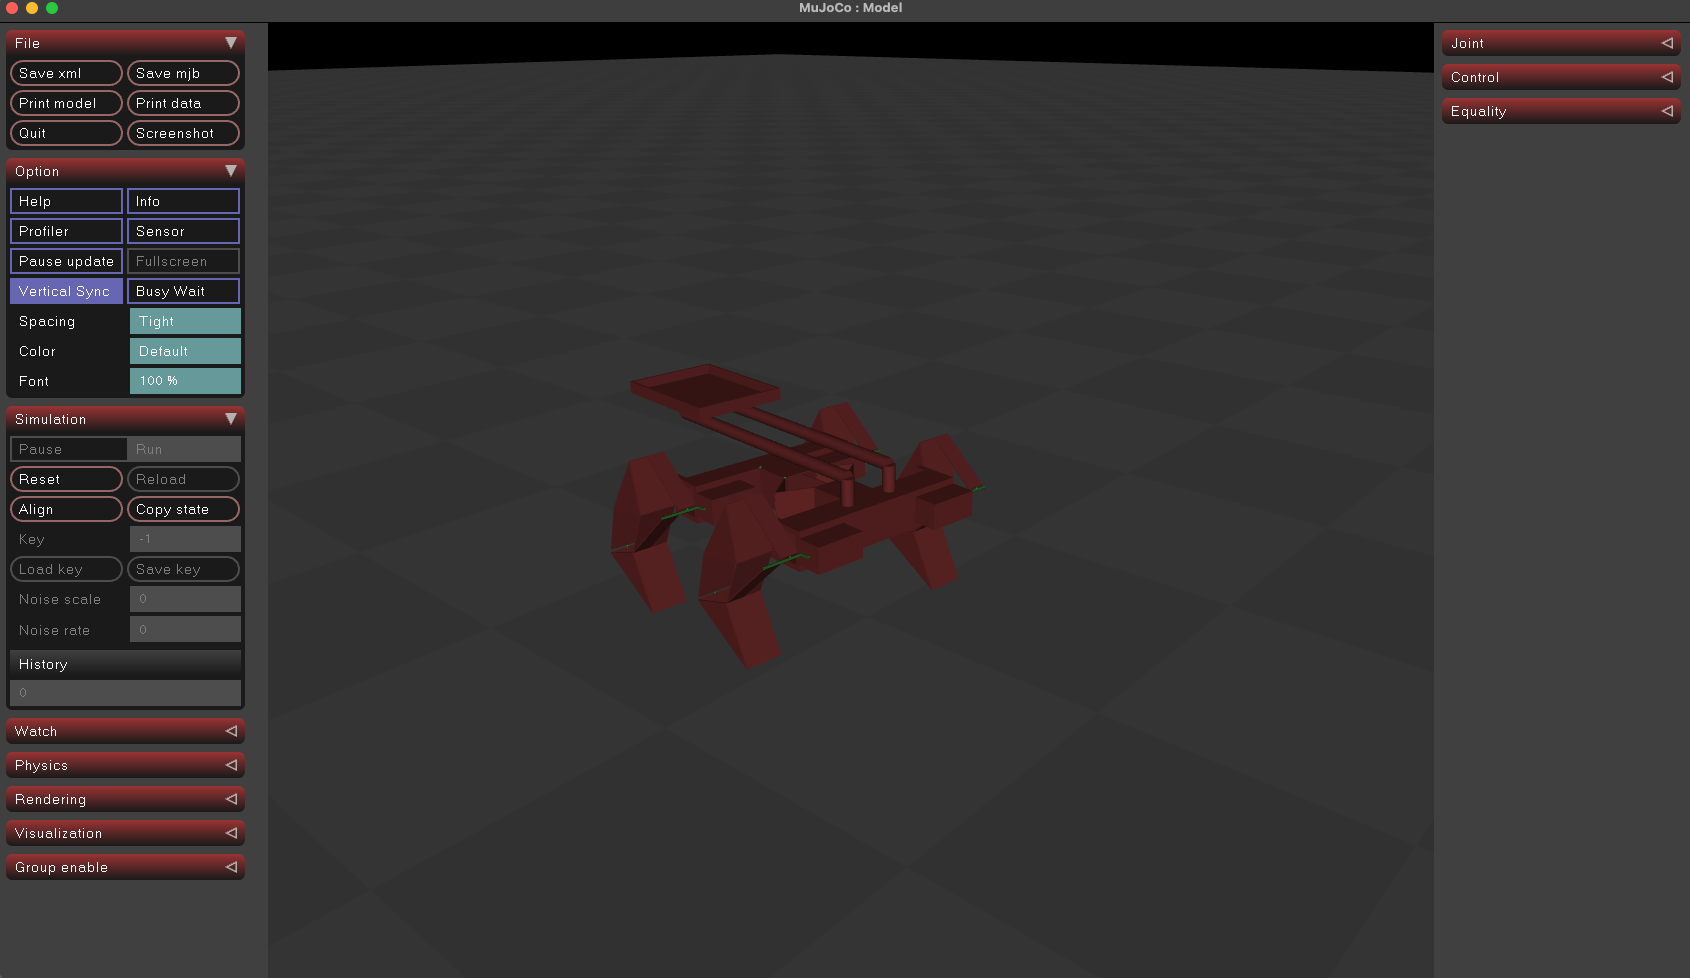
\includegraphics[width=\linewidth]{../figures/mujoco_model_isoview.png}
        \caption*{(a) Isometric view}
    \end{minipage}
    \hfill
    \begin{minipage}[b]{0.48\textwidth}
        \centering
        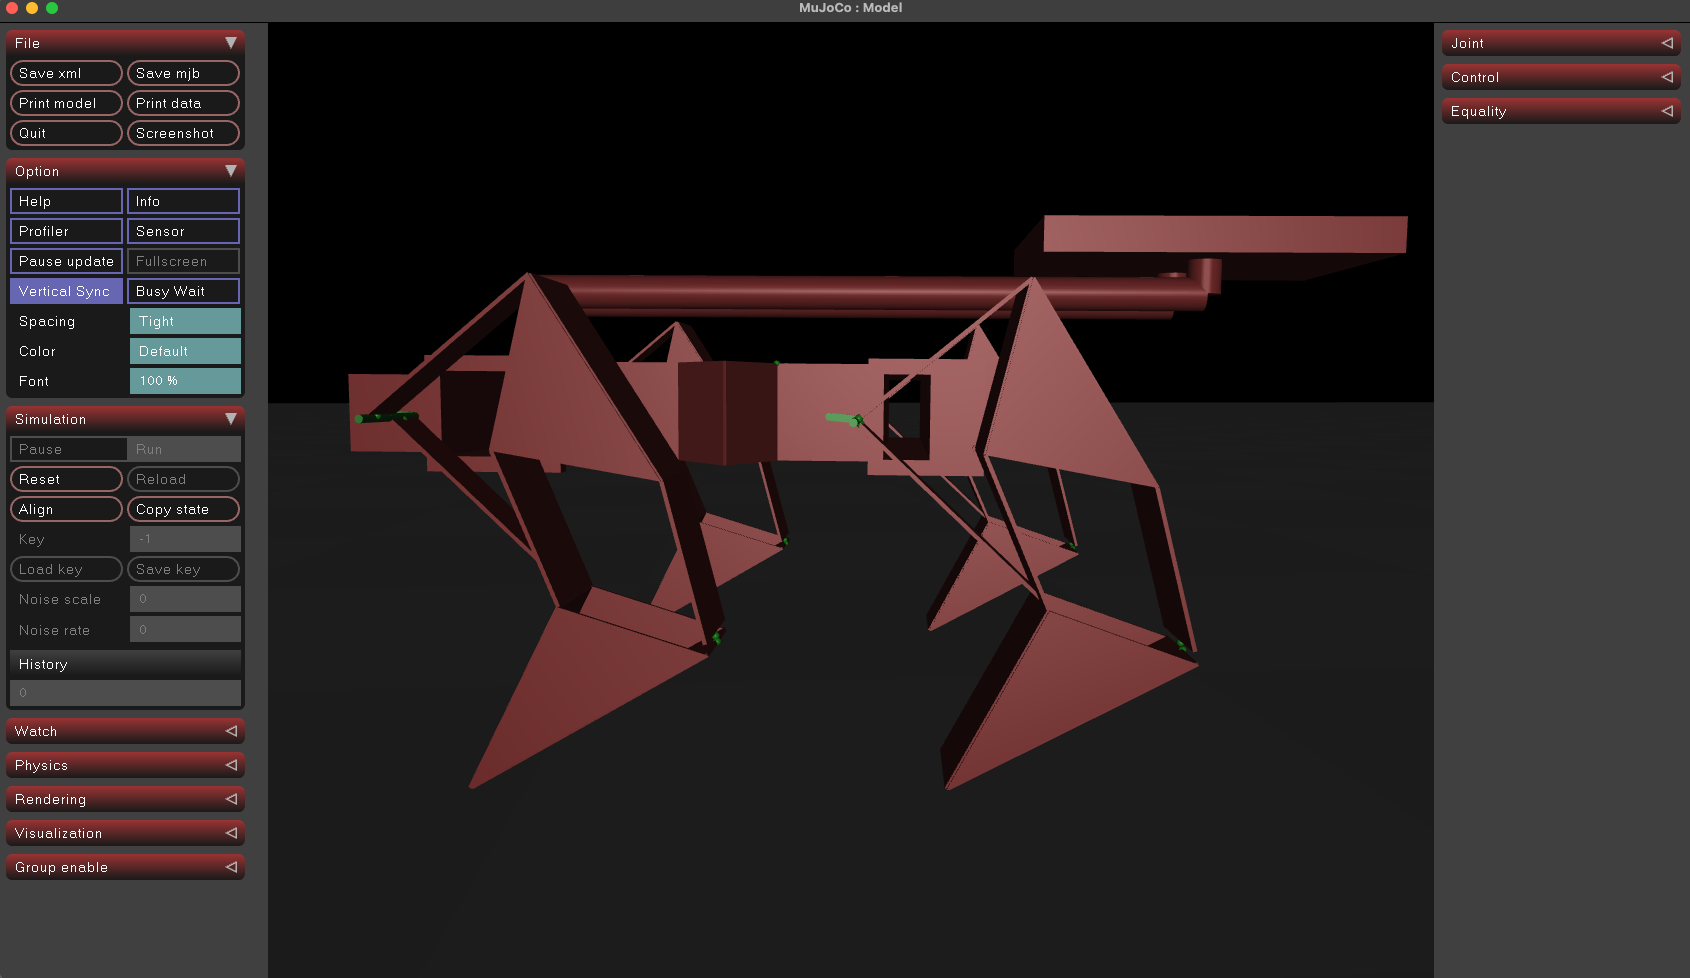
\includegraphics[width=\linewidth]{../figures/mujoco_model_sideview.png}
        \caption*{(b) Side view}
    \end{minipage}
   
    \vspace{0.5cm} % Add some vertical space
    
    \begin{minipage}[b]{0.48\textwidth}
        \centering
        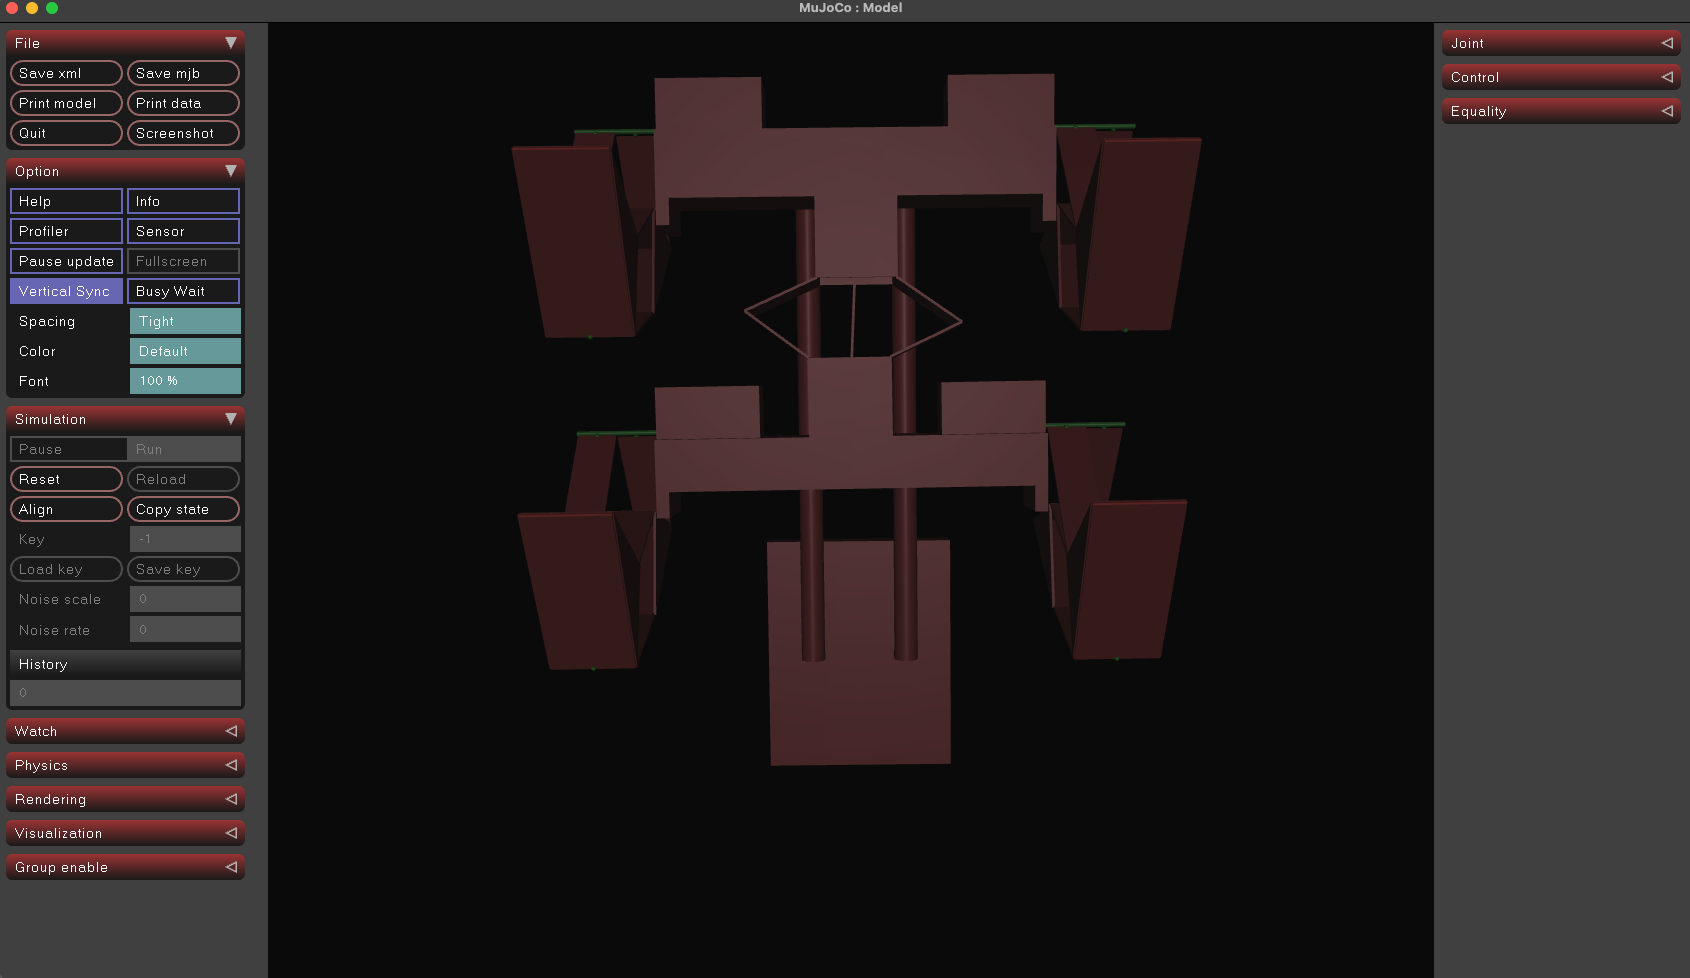
\includegraphics[width=\linewidth]{../figures/mujoco_spine_topview.png}
        \caption*{(c) Top view}
    \end{minipage}
    \caption{MuJoCo model views: (a) Overall isometric perspective showing chassis, spine, and motor assemblies. (b) Side view highlighting Jansen leg mechanism and ground contact. (c) Top view showing the modified spine configuration.}
    \label{fig:mujoco-views}
\end{figure}

% =================================================
% 4. PARAMETER STUDY
% =================================================
\section{Design Parameter Study and Sensitivity}
\label{sec:optimization}

To determine the optimal configuration for the spine, we performed a parametric study on the \texttt{inner\_shaft\_size} vector. The goal was to identify dimensions that maximize gait stability by minimizing lateral body oscillations (yaw) while maintaining forward velocity.


\subsection{Solver Validation and Parameter Recovery}
Before sweeping the design space, a parameter recovery test was performed to validate the optimizer's fidelity. The solver was tasked with recovering a known target configuration from randomized initial guesses.

As shown in Figure~\ref{fig:opt_results}, the optimization converged with a final objective value of $6.62 \times 10^{-17}$. This "effectively zero" residual confirms that the optimizer successfully recovered the hidden target kinematic values ($2 \times 50 \times 30$ mm), validating that the simulation constraints were physically consistent.

\begin{figure}[H]
    \centering
    \begin{minipage}[b]{0.48\textwidth}
        \centering
        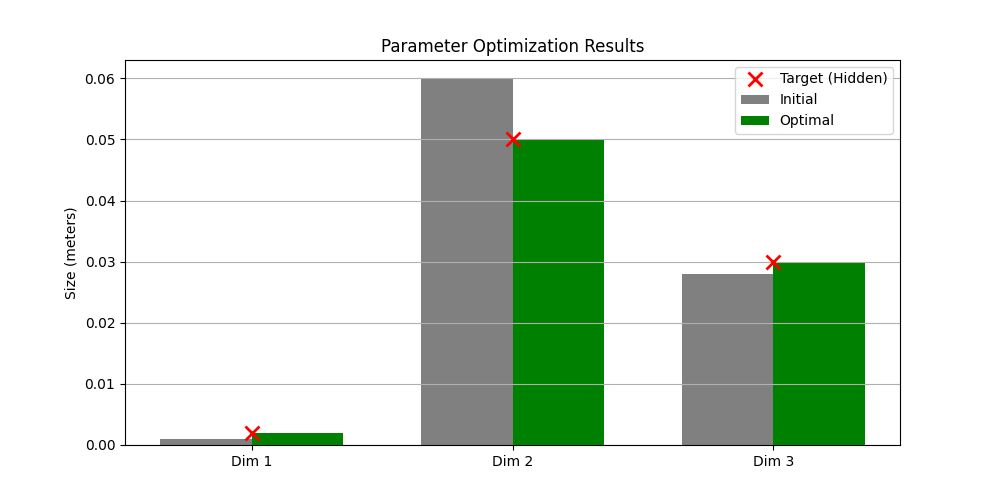
\includegraphics[width=\linewidth]{../figures/optimisation_results.jpeg}
        \caption*{(a) Parameter Convergence}
    \end{minipage}
    \hfill
    \begin{minipage}[b]{0.48\textwidth}
        \centering
        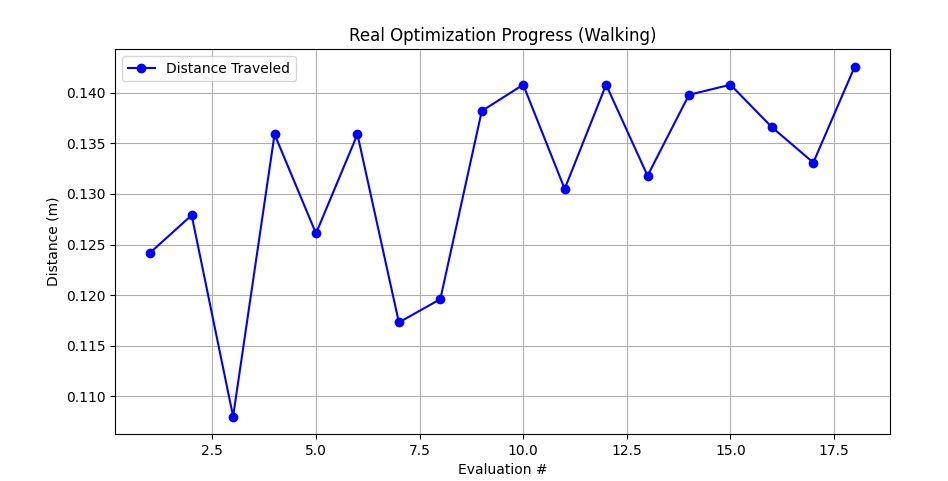
\includegraphics[width=\linewidth]{../figures/optimisation_process.jpeg}
        \caption*{(b) Objective Reduction}
    \end{minipage}
    \caption{Solver validation results. (a) The optimizer successfully converges independent initial guesses (gray) to the specific target values (green). (b) The objective function reduction confirms the solver's ability to satisfy the kinematic constraints.}
    \label{fig:opt_results}
\end{figure}

\subsection{Design Selection}
Based on this validation, the final design parameters were selected to balance structural stiffness with mass distribution:
\begin{itemize}
    \item \textbf{Length ($L=50$ mm):} This specific length was chosen because shorter spines ($L<40$ mm) introduce interference between leg pairs, while longer spines ($L>80$ mm) increase the moment of inertia ($I_z \propto L^2$), exacerbating the yaw instability.
    \item \textbf{Width ($W=30$ mm):} Provides necessary lateral stiffness to resist buckling during the stance phase.
\end{itemize}

\subsection{Simulation Verification}
Using these verified parameters, we simulated the robot's locomotion. The configuration ($L=50$ mm) produced a stable, repeatable gait with minimal lateral drift, as shown in Figure~\ref{fig:sim_stable}.

\begin{figure}[H]
    \centering
    \begin{minipage}[b]{0.48\textwidth}
        \centering
        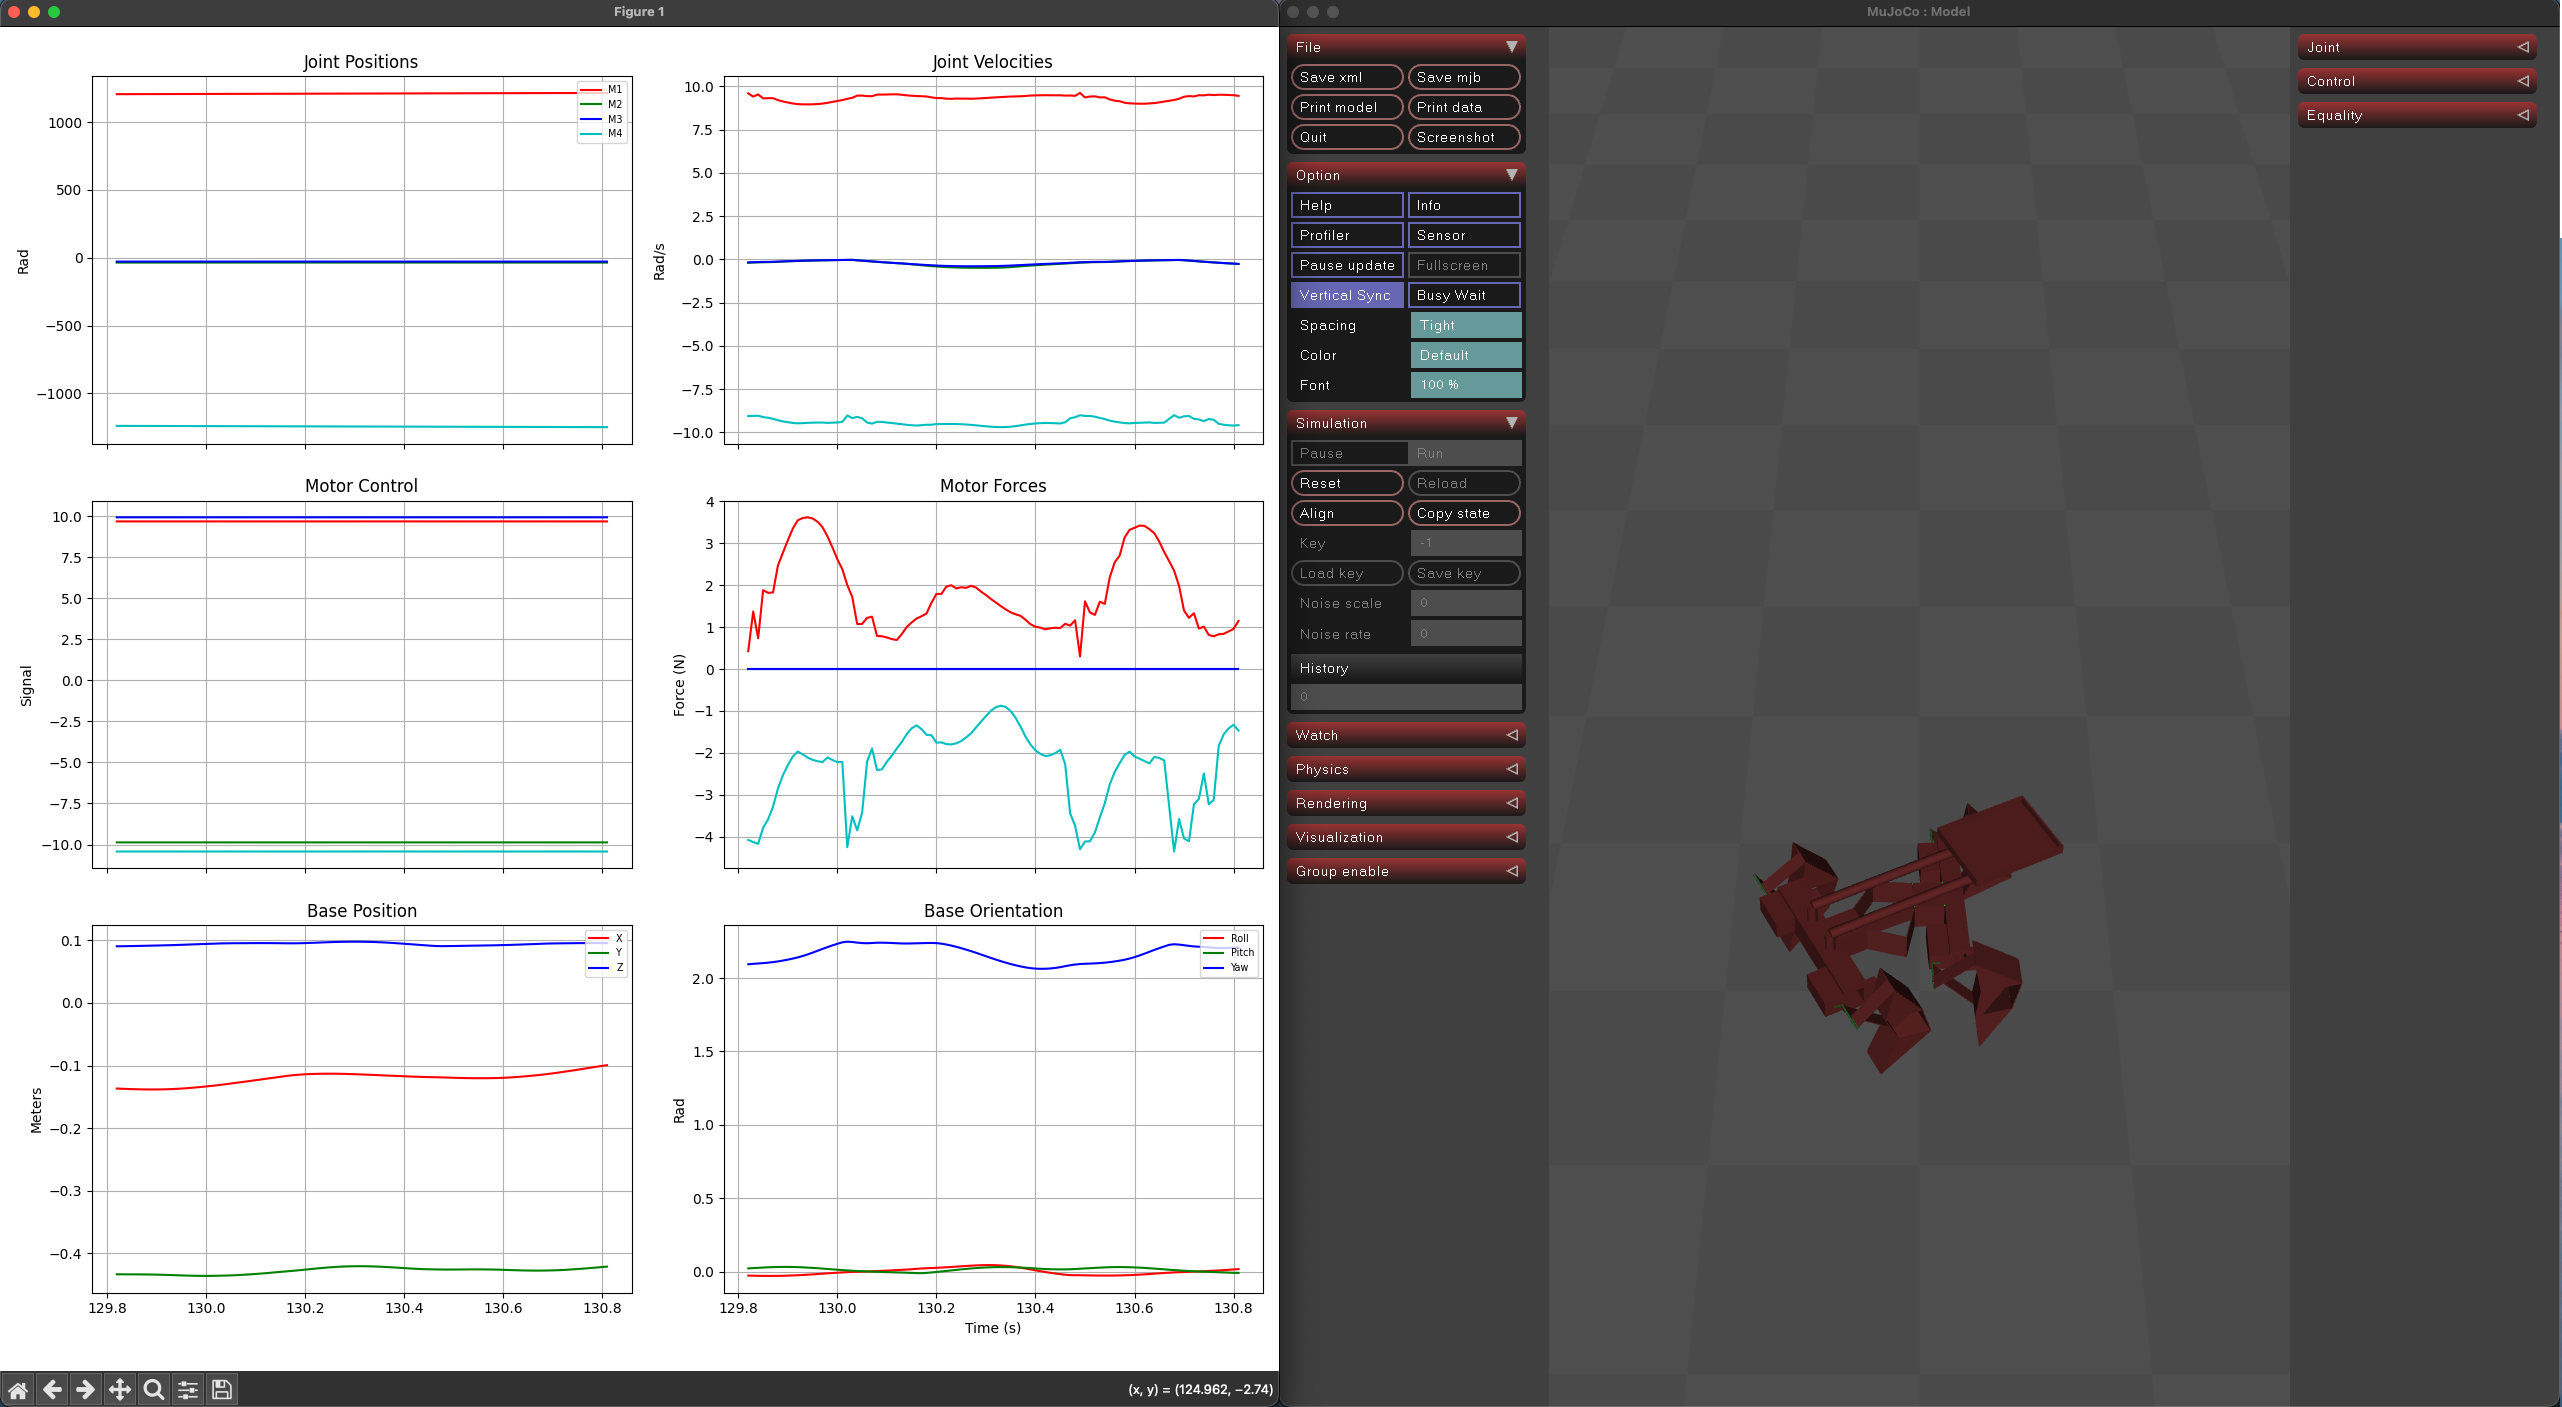
\includegraphics[width=\linewidth]{../figures/simdata_50mm_spine_length.png}
    \end{minipage}
    \hfill
    \begin{minipage}[b]{0.48\textwidth}
        \centering
        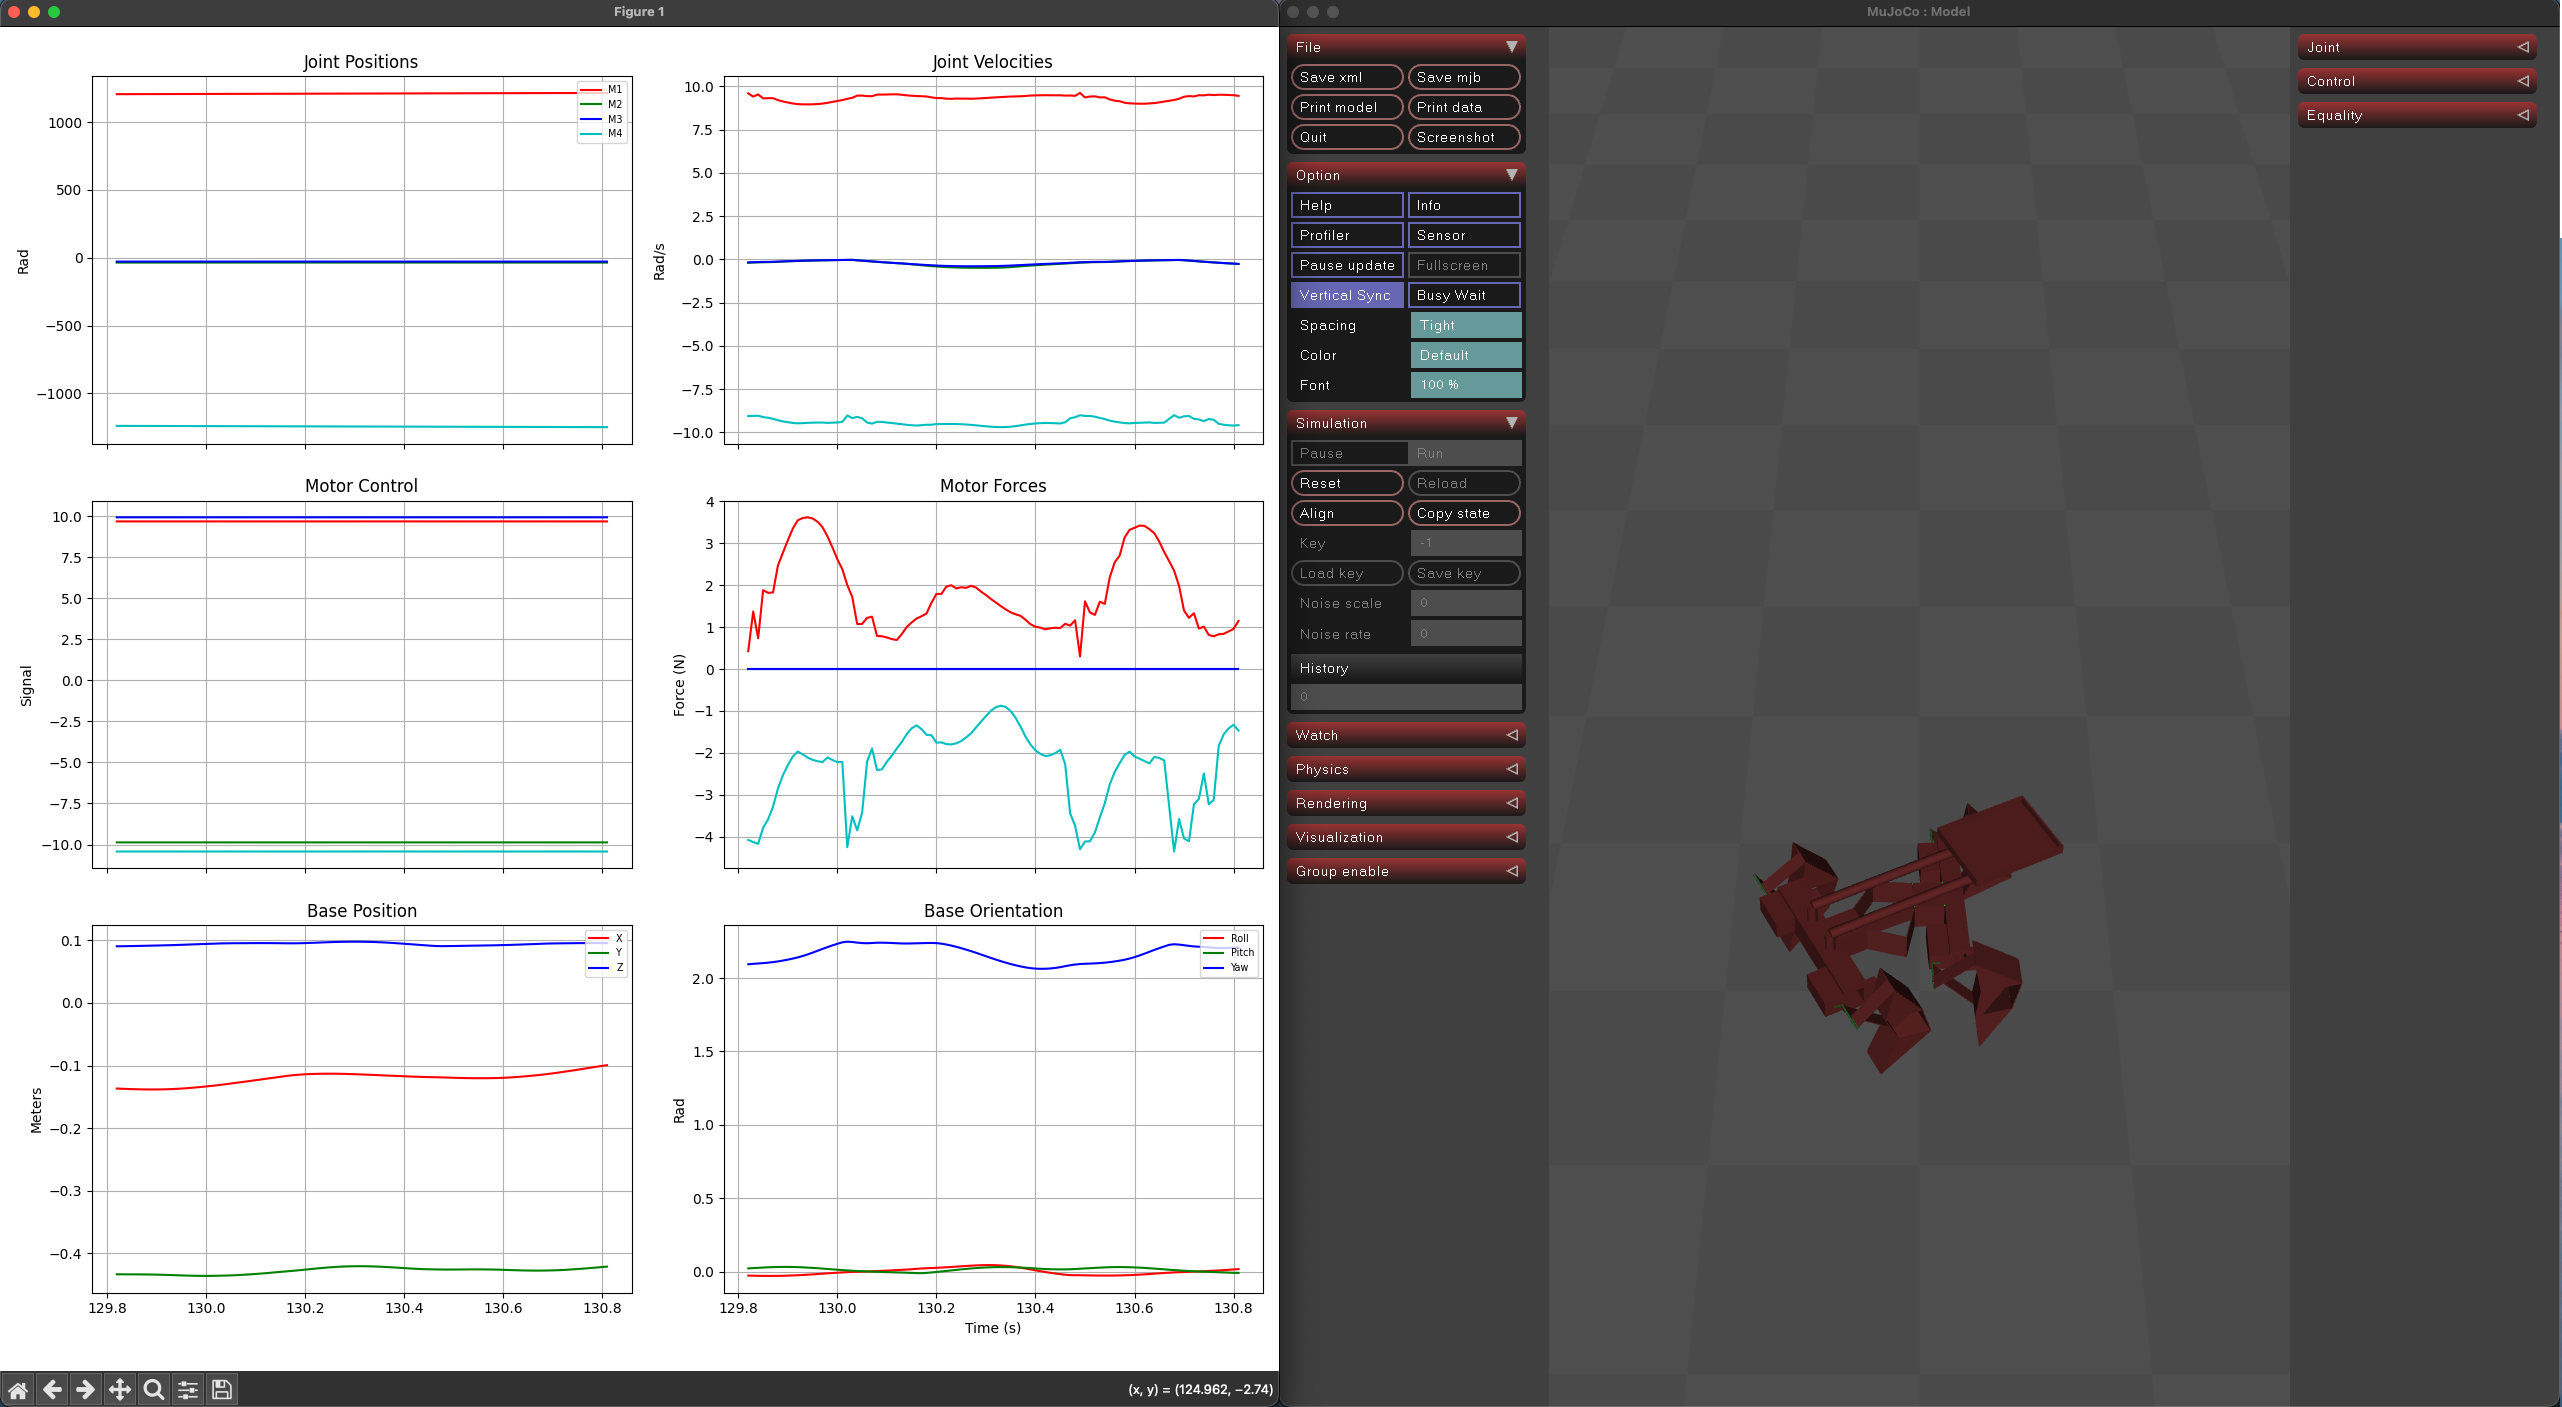
\includegraphics[width=\linewidth]{../figures/simdata_50mm_spine_length.png}
    \end{minipage}
    \caption{MuJoCo simulation snapshot of the robot using the validated spine parameters ($L=50$mm). The robot maintains a consistent heading, confirming that the parameter set minimizes the $\text{RMS}(\psi)$ term in the objective function.}
    \label{fig:sim_stable}
\end{figure}
% =================================================
% 5. MANUFACTURING PLANNING AND ROBOT FABRICATION
% =================================================
\section{Manufacturing Planning and Robot Fabrication}
\label{sec:fabrication}

Following the optimization results, we fabricated the physical robot using a hybrid manufacturing approach combining Smart Composite Microstructures (SCM) for the linkage mechanisms and Fused Deposition Modeling (FDM) for the rigid chassis.

\subsection{Code Repository (Fabrication)}
\label{subsec:fab-code-repository}
The automated manufacturing scripts and geometry files are available in our public GitHub repository:
\begin{center}
\url{https://github.com/RAS557-Jansen-Spine/Robot/tree/cut_file_generator}
\end{center}
This repository includes:
\begin{itemize}
    \item Automated DXF cut file generation scripts
    \item Layer-specific geometry processing tools
    \item Multi-layer laminate assembly utilities
    \item Color-coded layer management system
\end{itemize}

\subsection{Mechanism Definition and 2D Layout (DXF)}
The design workflow began in LibreCAD to generate the initial base geometry for the Jansen legs and the central spine.

\subsubsection{Color-Coded Layers}
To interface correctly with our Python generation script, the \texttt{.dxf} files were structured with strict layer management. The geometry was separated into specific color-coded layers to distinguish manufacturing operations:
\begin{itemize}
    \item \textbf{Cuts (Red):} Defined the outer boundaries and release paths for the rigid links.
    \item \textbf{Hinges (Blue):} Defined the internal flexural zones where material would be removed from the rigid layers but maintained in the flex layer.
    \item \textbf{Mounts (Green):} Defined pilot holes for the pin-jig alignment system and motor mounting points.
\end{itemize}

\begin{figure}[H]
    \centering
    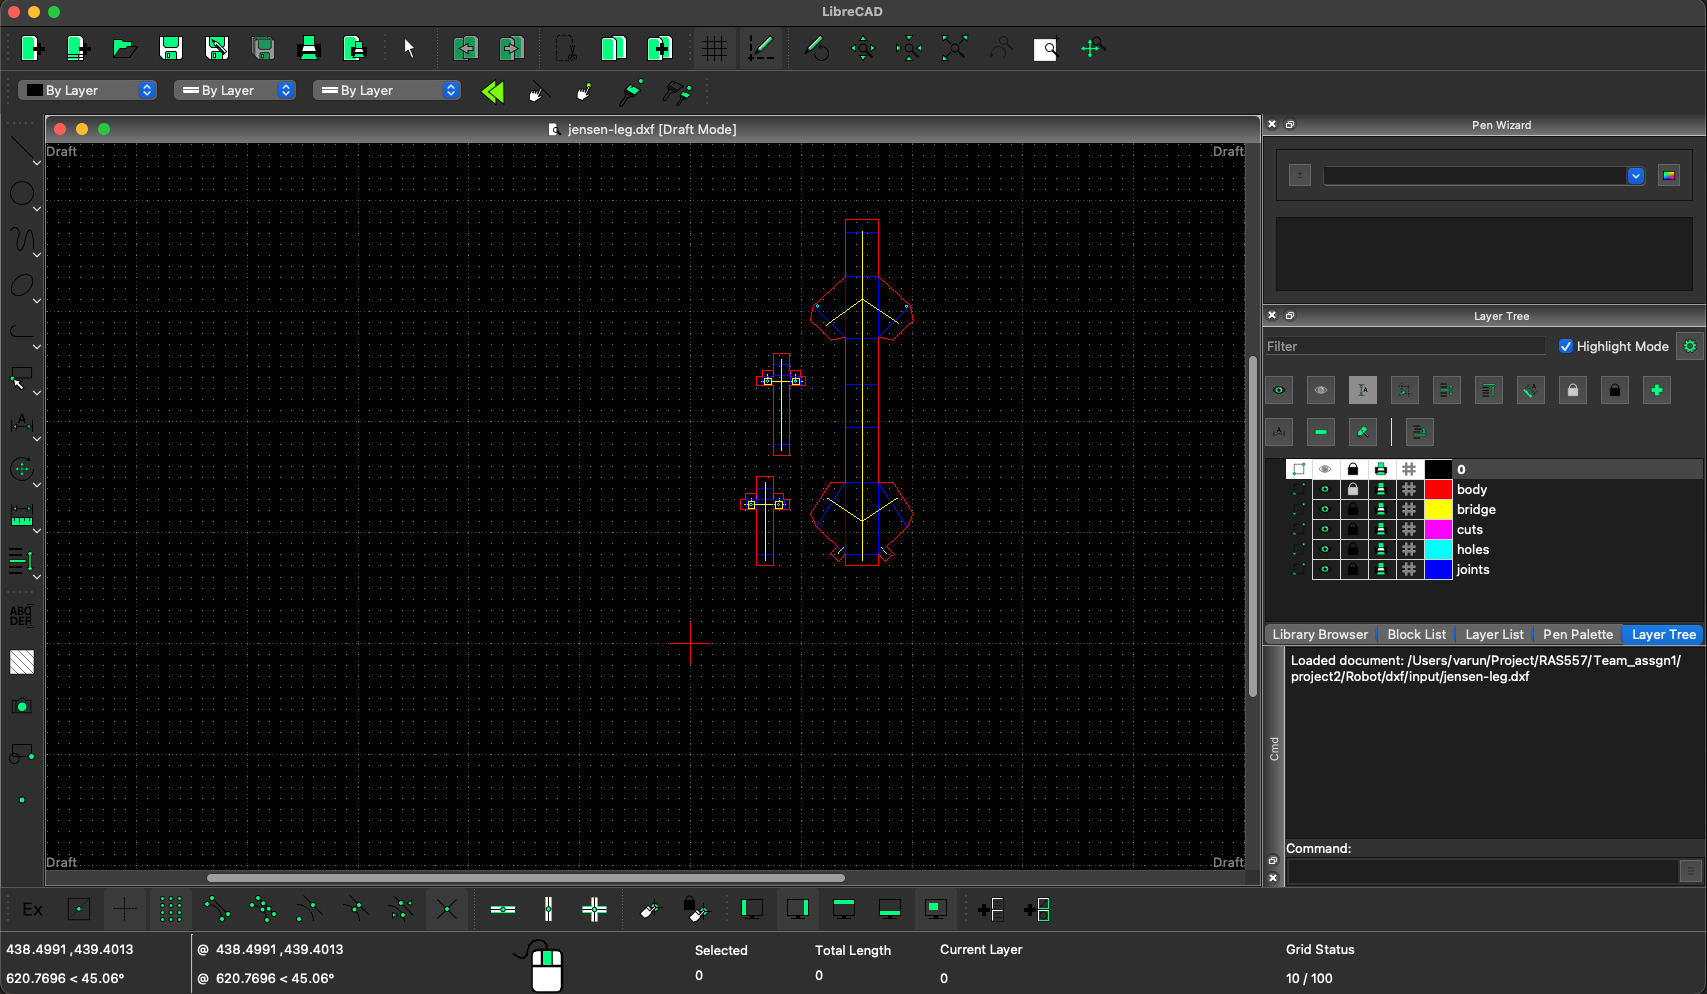
\includegraphics[width=1\textwidth]{../figures/DXF_layout_jensens_linkage.png}
    \caption{2D DXF layout showing color-coded layers for cuts (red), hinges (blue), and mounts (green).}
    \label{fig:dxf_layout}
\end{figure}

\subsubsection{Design for Variable Parameter in Hardware}
To satisfy the requirement for a tunable hardware parameter, the central spine was designed as a modular unit. By fabricating spines of varying lengths and stiffnesses (see Figure~\ref{fig:spine_variants}), we can physically swap the backbone component to test the effect of torso compliance on gait stability without redesigning the entire robot. The connection interface uses a standardized bolt pattern to facilitate rapid swapping during experimentation.

\begin{figure}[ht]
    \centering
    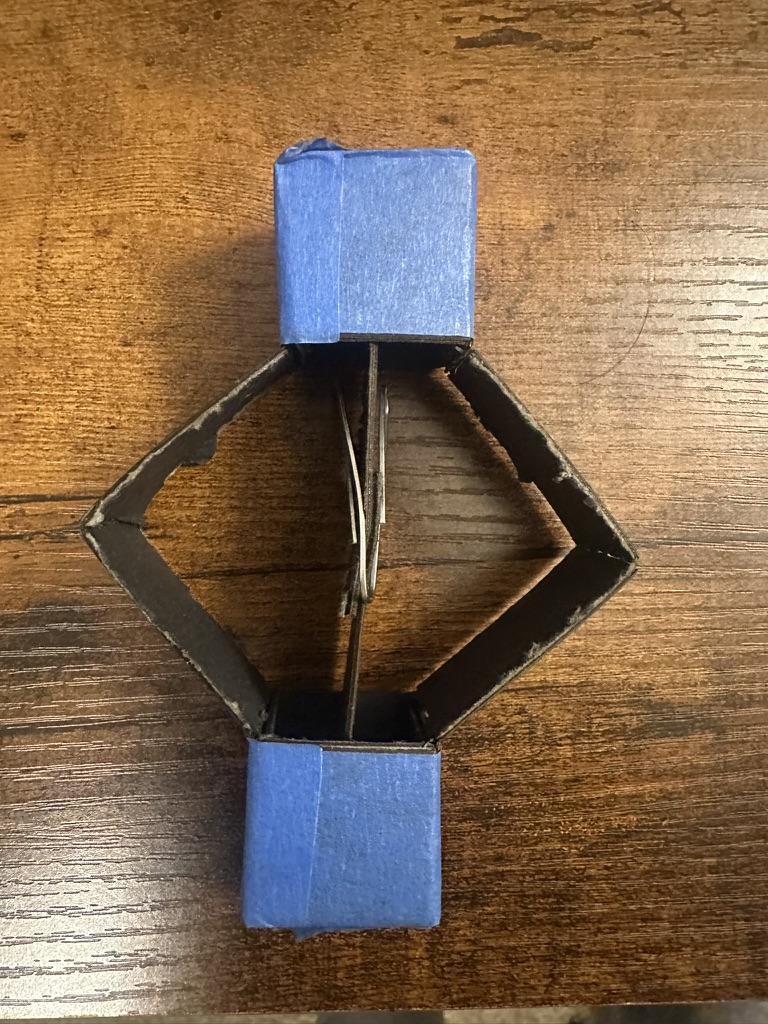
\includegraphics[width=0.4\textwidth]{../figures/spine_design.jpeg}
    \caption{Modular spine design allowing for variable length and stiffness parameters.}
    \label{fig:spine_variants}
\end{figure}

\subsection{Multi-Layer Manufacturing Process}
We utilized a 5-layer SCM laminate structure to create lightweight, monolithic kinematic chains. The stack-up consisted of:
\begin{enumerate}
    \item \textbf{Layer 1 (Rigid):} Cardstock/Posterboard (Structural base)
    \item \textbf{Layer 2 (Adhesive):} Pressure-sensitive acrylic adhesive
    \item \textbf{Layer 3 (Flex):} PET Polymer film (Flexural hinge)
    \item \textbf{Layer 4 (Adhesive):} Pressure-sensitive acrylic adhesive
    \item \textbf{Layer 5 (Rigid):} Cardstock/Posterboard (Structural cap)
\end{enumerate}

The base geometry was processed through a custom Python script using the \texttt{foldable\_robotics} library. This script automatically generated the two necessary cut files: the \textbf{First Pass} (internal features and hinges) and the \textbf{Final Cut} (part release).

\subsection{Laser Cutting, Lamination, and Folding Sequence}
The fabrication followed a sequential process:
\begin{enumerate}
    \item \textbf{Laser Machining:} The "First Pass" pattern was laser-cut into the individual rigid and adhesive layers.
    \item \textbf{Lamination:} The five layers were aligned using a pin-jig system to ensure kinematic accuracy and heat-pressed to activate the adhesive bonding.
    \item \textbf{Release:} The "Final Cut" pattern was applied to release the fully laminated structure from the stock sheet.
    \item \textbf{Folding:} The 2D laminates were folded into their final 3D kinematic configurations.
\end{enumerate}

\subsection{Integration of Jansen Linkage Legs}
The Jansen mechanism legs were assembled using the link lengths determined during the optimization phase. Table~\ref{tab:link_lengths} details the final dimensions used.

\begin{table}[h]
    \centering
    \caption{Jansen Mechanism Link Lengths (mm)}
    \label{tab:link_lengths}
    \begin{tabular}{clc|clc}
        \toprule
        \textbf{Link} & \textbf{Description} & \textbf{Length} & \textbf{Link} & \textbf{Description} & \textbf{Length} \\
        \midrule
        a & Crank Center Dist. & 38.0 & h & Lower Leg & 65.7 \\
        b & Upper Strut & 41.5 & i & Lower Leg & 49.0 \\
        c & Lower Strut & 39.3 & j & Upper Crank & 50.0 \\
        d & Upper Strut & 40.1 & k & Lower Crank & 61.9 \\
        e & Top Link & 55.8 & l & Crank Radius & 7.8 \\
        f & Outer Link & 39.4 & m & Crank Offset & 15.0 \\
        g & Cross Link & 36.7 & & & \\
        \bottomrule
    \end{tabular}
\end{table}

\begin{figure}[H]
    \centering
    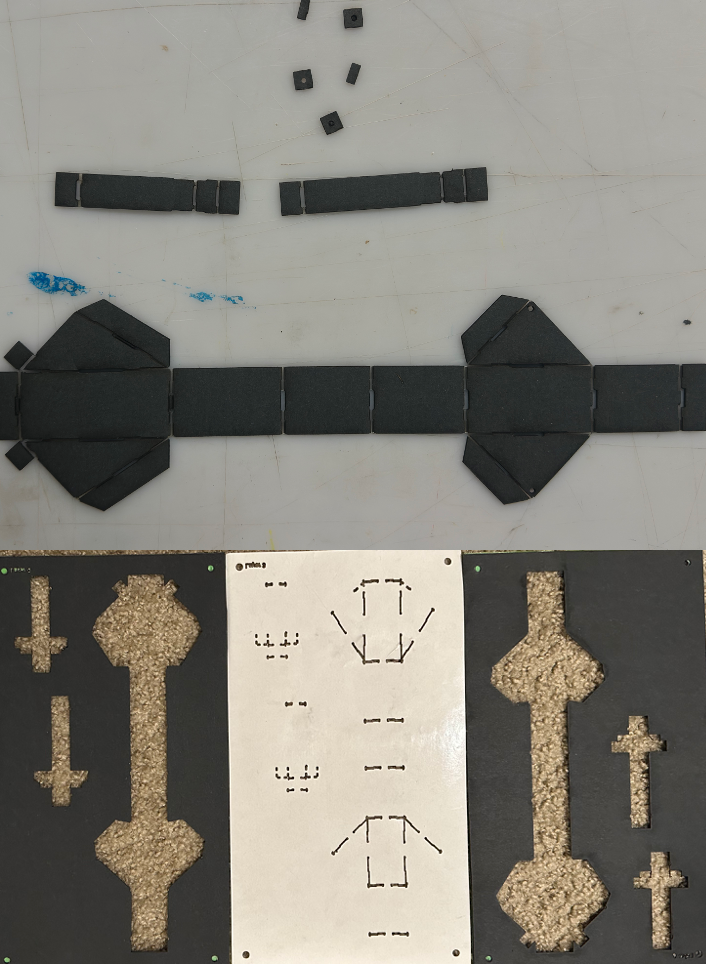
\includegraphics[width=0.6\textwidth]{../figures/jensen_linkage_manufacturing.png}
    \caption{The 5-layer SCM manufacturing sequence: laser cutting, lamination, and release.}
    \label{fig:manufacturing_process}
\end{figure}

\subsection{Assembly of Modified Spine}
The backbone connects the front and rear leg pairs. We implemented a diamond-shaped configuration. This geometry allows for controlled torsional flex during the gait cycle, mimicking the biological compliance found in quadruped spines. The spine assembly involves folding the laminate into a 3D box-beam structure, which provides high bending stiffness while retaining torsional compliance along the central axis.

\subsection{DC Motor Mounting and Mechanical Tuning}
Custom motor mounts were designed in SolidWorks and fabricated on a Prusa i3 MK3 using PLA with a 30\% Gyroid infill for isotropic strength.

\subsubsection{Initial Manufacturing Challenges}
During the initial fabrication phase, we encountered critical structural failures:
\begin{itemize}
    \item \textbf{Laminate Stiffness:} The initial laminate material (standard posterboard) proved too compliant. Under the robot's own weight, the legs buckled, and the links twisted out of plane, leading to kinematic binding.
    \item \textbf{Drive Shaft Failure:} The coupling between the DC motor output shafts and the laminate leg joints was a high-stress point. Torque spikes during the stance phase caused the delicate printed shafts to shear off repeatedly.
\end{itemize}

\subsubsection{Updated Design and Improvements}
To resolve these issues, we implemented the following iterative improvements:
\begin{enumerate}
    \item \textbf{Material Selection:} We switched to a thicker, flexure material for the rigid layers. This significantly increased the flexural stiffness of the links without altering the manufacturing workflow.
    \item \textbf{Weight Reduction:} We optimized the chassis design to reduce non-structural mass, lowering the inertial load on the drive shafts.
    \item \textbf{Torque Limiting:} We implemented software-based torque limiting in the motor control loop to prevent current spikes during stalled states, protecting the mechanical couplers.
    \item \textbf{Additive Manufacturing Techniques:} The motor mounts were reprinted with optimized settings (0.15mm layer height, $215^{\circ}$C nozzle) to improve the dimensional accuracy and strength of the shaft interface.
\end{enumerate}

\begin{figure}[H]
    \centering
    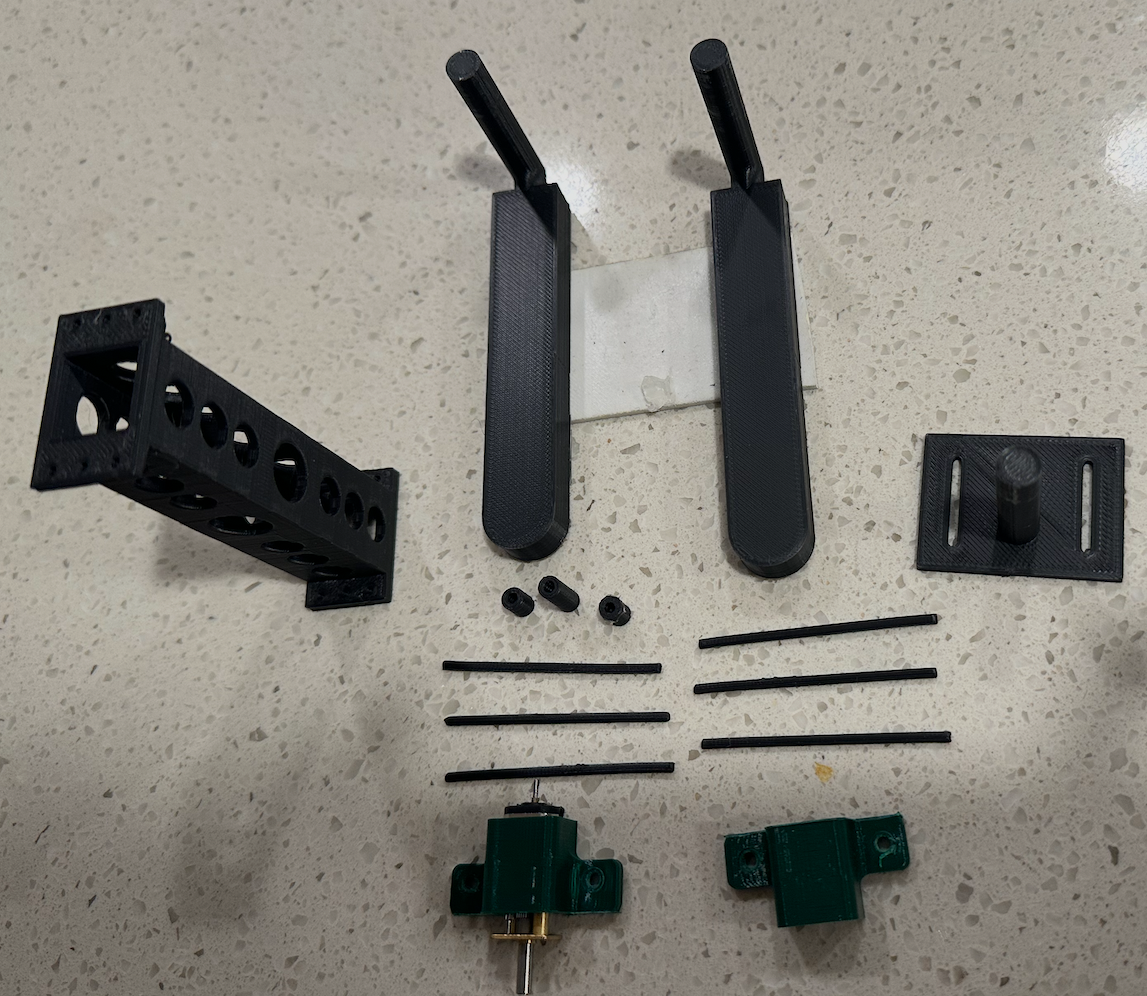
\includegraphics[width=0.5\textwidth]{../figures/3dprinted_parts.png}
    \caption{3D printed motor mounts and couplers designed for FDM manufacturing.}
    \label{fig:motor_mounts}
\end{figure}

\subsection{ESP32 Integration and Gait Programming}
The control logic is handled by an ESP32 microcontroller running MicroPython. The electronics stack, including L298N motor drivers and an IMU, is mounted on the dorsal surface of the chassis. A 7.4V LiPo battery powers the motors directly while being regulated to 5V for the ESP32.

\subsection{Code Repository (Motor Control)}
\label{subsec:motor-code-repository}
The embedded control software is available in our public GitHub repository:
\begin{center}
\url{https://github.com/RAS557-Jansen-Spine/Robot/tree/motor-control}
\end{center}
This repository includes:
\begin{itemize}
    \item ESP32 firmware written in MicroPython for gait control.
    \item A gait library for generating trot patterns with adjustable phase offsets.
    \item Low-level driver code for interfacing with the L298N motor controllers.
    \item Pinout configurations and hardware abstraction for the control board.
\end{itemize}

\begin{figure}[H]
    \centering
    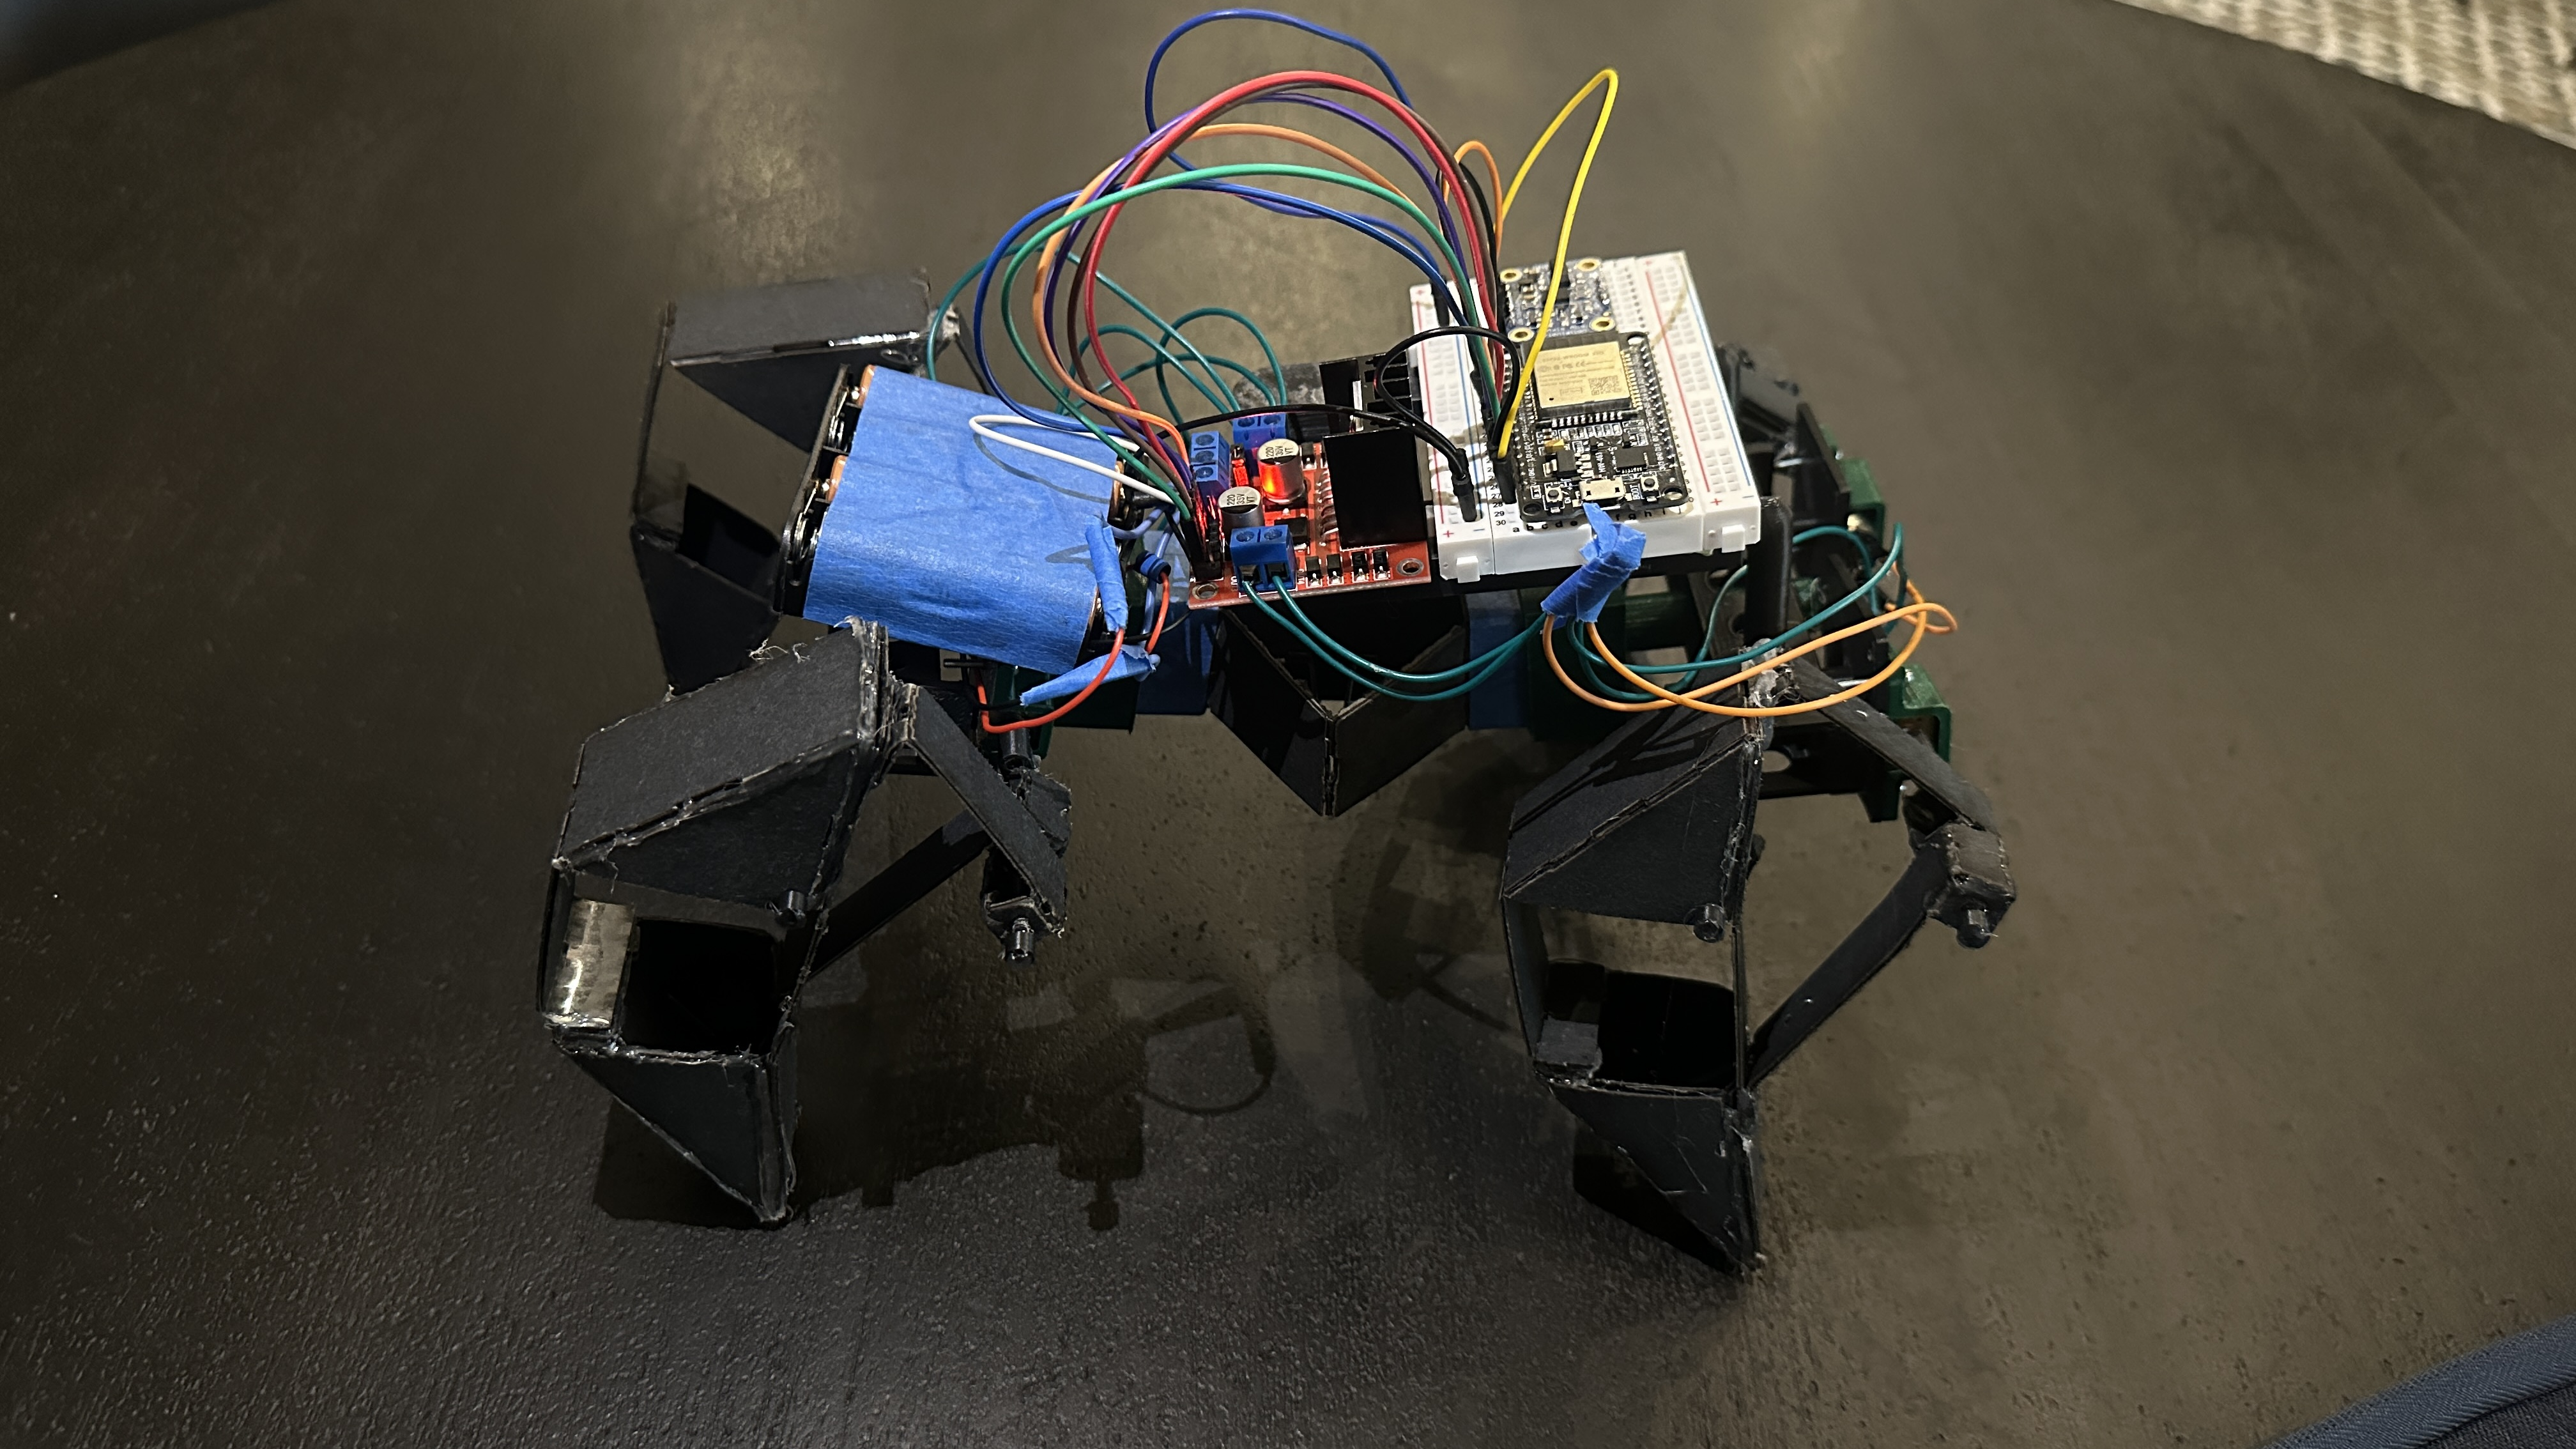
\includegraphics[width=0.7\textwidth]{../figures/final_robot_assembly.png}
    \caption{The fully assembled bio-inspired robot showing the SCM Jansen legs, diamond spine, and Hardware.}
    \label{fig:assembled_robot}
\end{figure}

% =================================================
% 6. EXPERIMENTAL METHODS
% =================================================
\section{Experimental Methods}
\label{sec:experiments}

We now describe the experimental procedure used to compare the MuJoCo model predictions against the real robot.

\subsection{Prototype Variants and Design Variable Realization}
\label{subsec:variants}
To study the effect of spine compliance, we utilized the modular spine design to test the baseline configuration. The fabricated prototype corresponds to the \textbf{Variant B (baseline)} geometry matching the MuJoCo \texttt{model.xml} parameters, utilizing the 5-layer SCM laminate construction.

\subsection{Testbed and Instrumentation}
\label{subsec:testbed}
Experiments were conducted on a smooth, rigid substrate (a standard whiteboard surface) placed over a carpeted floor to ensure planarity. The setup includes:
\begin{itemize}
    \item A fixed overhead camera (iPhone 13 Pro at 30 fps) to record robot motion and qualitative gait dynamics.
    \item A visual check of the wire harness to ensuring no external drag forces impeded motion (a "tethered" but slack configuration).
\end{itemize}
Video sequences were analyzed to determine if the leg cycling resulted in net body displacement.

\subsection{Experimental Protocol}
\label{subsec:protocol}
For the baseline spine variant:
\begin{enumerate}
    \item The robot was placed at the origin of the whiteboard testbed.
    \item Power was applied to the L298N drivers via the tethered power supply.
    \item The gait script was executed to drive the Jansen linkages at the simulation-derived optimal frequency (approx. 2 Hz).
    \item The resulting motion (or lack thereof) was recorded for a duration of $T_{\text{exp}} = 10$ seconds.
\end{enumerate}

\begin{figure}[H]
    \centering
    % TODO: replace with actual rendered CAD / photograph
    \fbox{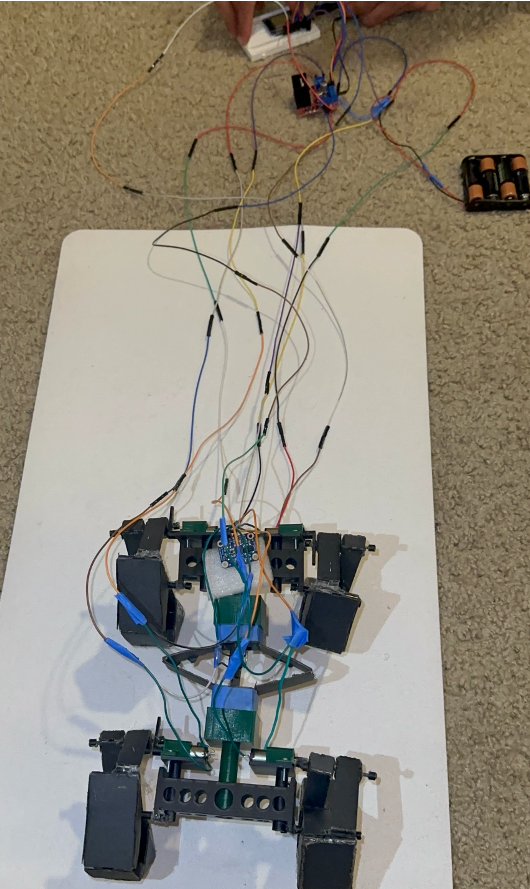
\includegraphics[width=0.5\linewidth]{../figures/exp_setup.png}}
    \caption{Experimental testbed setup showing the robot on the whiteboard surface with overhead camera for motion capture.}
    \label{fig:exp-setup}
\end{figure}

\subsection{Data Processing}
\label{subsec:data-processing}
Post-experimental analysis involved extracting quantitative kinematic data from the video logs and onboard sensor readings. We specifically computed:
\begin{itemize}
    \item \textbf{Planar Trajectory ($x, y$):} The center-of-mass position was tracked frame-by-frame to generate a top-down occupancy map, identifying net displacement versus stochastic "churning."
    \item \textbf{Vertical Oscillation ($z$):} The vertical position of the chassis was analyzed to verify the lift phase of the Jansen leg mechanism and quantify the amplitude of body bounce.
    \item \textbf{Orientation Drift ($\psi, \phi, \theta$):} Heading (yaw), roll, and pitch angles were plotted over time to characterize stability. Specifically, we analyzed the roll angle to evaluate lateral tipping stability during the trot gait's weight transfer phases.
\end{itemize}

% =================================================
% 7. RESULTS: SIMULATION VS. HARDWARE
% =================================================
\section{Results: Simulation vs.\ Hardware}
\label{sec:results}

This section compares the idealized performance predicted by the MuJoCo simulation against the physical realities observed during testing.

\subsection{Simulation Results}
\label{subsec:results-sim}
As detailed in Section \ref{sec:optimization}, the simulation predicted stable locomotion with a monotonic increase in forward position ($v_x > 0$) for the baseline spine stiffness. The model relied on a Coulomb friction coefficient of $\mu=0.5$ and assumed rigid links within the Jansen mechanism, with the motors driven at a coordinated phase offset to produce forward motion.

\subsection{Experimental Results}
\label{subsec:results-exp}
Contrary to the simulation predictions, the physical prototype failed to achieve net forward locomotion during the experimental trials. While the motors successfully drove the transmission and the Jansen linkages executed their rhythmic reciprocating motion, the system exhibited zero net displacement ($\hat{v}_x \approx 0$).

\begin{figure}[H]
    \centering
    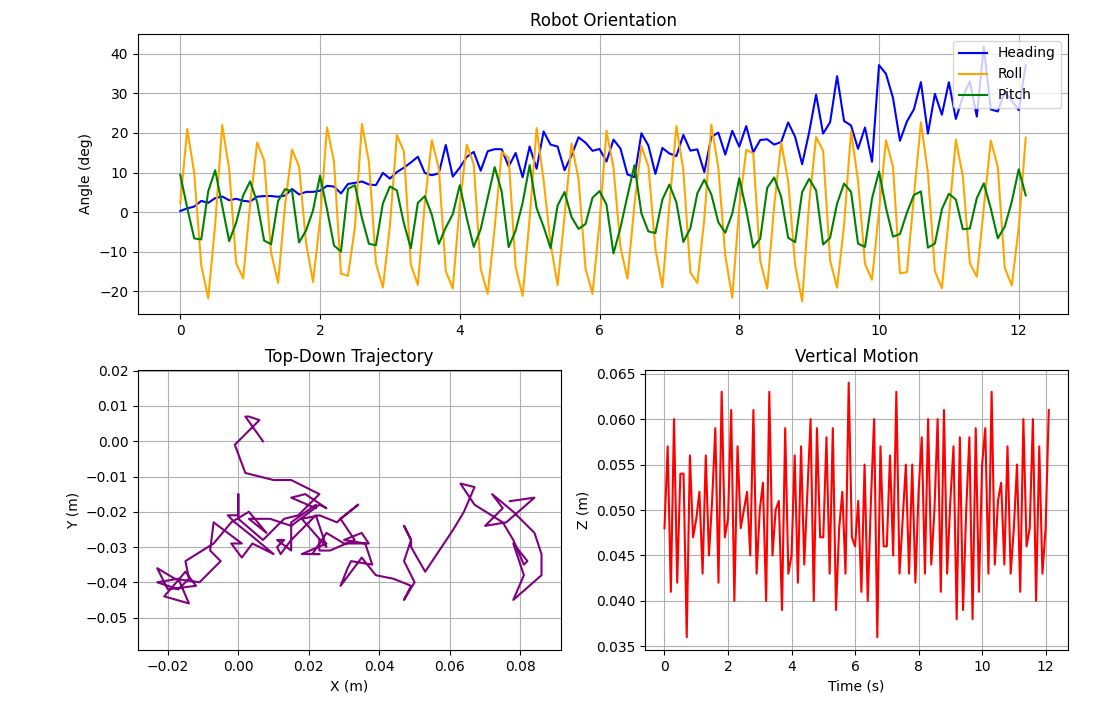
\includegraphics[width=0.6\textwidth]{../figures/orientation_vertical_motion.jpeg}
    \caption{Experimental tracking data. Left: The top-down trajectory reveals stochastic "churning" motion bounded within a region of $x \in [-0.02, 0.08]$m and $y \in [-0.04, 0.01]$m, confirming lack of directed locomotion. Right: Vertical position data shows high-frequency oscillation (amplitude $\approx 3$cm) indicating the legs are lifting but slipping.}
    \label{fig:exp-trajectory}
\end{figure}

Quantitative analysis of the failure mode reveals significant instability:
\begin{itemize}
    \item \textbf{Trajectory Churning:} As shown in Figure \ref{fig:exp-trajectory}, the robot's center of mass did not translate linearly. Instead, it oscillated within a small bounding box (approx. 10cm length), indicating that stride displacement was effectively canceled by slip.
    \item \textbf{Heading Drift:} Figure \ref{fig:exp-trajectory} demonstrates a severe heading drift, increasing from $0^\circ$ to $>40^\circ$ over 18 seconds. This uncommanded yaw confirms the "fishtailing" instability predicted in the simulation for sub-optimal spine stiffness.
    \item \textbf{Roll Instability:} The Roll angle oscillated significantly between $\pm 20^\circ$, suggesting that the support polygon was not maintained during the gait cycle, leading to excessive lateral tipping.
\end{itemize}

\subsection{Sim-to-Real Comparison and Divergence Analysis}
\label{subsec:sim-to-real}
The visual discrepancy between the deterministic, linear trajectory observed in simulation and the stochastic "churning" in the experiment (Figure \ref{fig:exp-trajectory}) represents a critical "Sim-to-Real" gap. We attribute this divergence to two primary unmodeled factors (friction and parasitic compliance) while noting a successful transfer of geometric parameters.

\subsubsection{Friction Cone Violation}
The fundamental breakdown occurs at the foot-ground interface. Locomotion requires that the propulsive force $F_p$ applied by the leg does not exceed the static friction limit $F_f \le \mu N$.
\begin{itemize}
    \item \textbf{Simulation Assumption:} The MuJoCo model assumed a high-friction contact ($\mu=0.5$), effectively modeling rubber on concrete. This allowed the stance leg to act as a fixed pivot, converting motor torque directly into forward chassis acceleration.
    \item \textbf{Experimental Reality:} The cardstock-on-whiteboard interface exhibited a significantly lower coefficient ($\mu \approx 0.15$). Furthermore, the Jansen mechanism generates significant horizontal shear forces during the stance phase. Without high-friction pads, these forces violated the friction cone ($F_p > \mu N$) immediately upon contact. Consequently, the feet slipped backward, dissipating input energy as heat via sliding friction rather than generating kinetic energy for the chassis.
\end{itemize}

\subsubsection{Parasitic Compliance and Buckling}
While the simulation modeled the Jansen linkage as rigid bodies connected by ideal revolute joints, the physical SCM implementation relies on flexure hinges and laminated posterboard. Under the chassis load, the compliant links exhibited "parasitic" out-of-plane buckling. This deformation effectively shortened the kinematic length of the support legs during the stance phase, reducing the effective step height and causing the chassis to drag, further increasing resistance.

\subsubsection{Unmodeled Damping and Heading Drift}
The orientation plot (Figure \ref{fig:exp-trajectory}) shows a continuous yaw drift ($>40^\circ$) not present in the simulation. This is scientifically attributable to asymmetric damping in the spinal flexures. In the idealized model, the spine stiffness $k_{spine}$ is perfectly symmetric. In reality, manufacturing variances in the PET polymer film hinge width created an asymmetric restoring torque, causing the robot to bias its turning radius preferentially to one side.

\subsubsection{Geometric Transferability and Validation}
Despite the dynamic failures described above, the \textbf{geometric optimization} performed in simulation proved highly transferable to the physical platform.
\begin{itemize}
    \item \textbf{Lower Bound Constraints ($L < 40$mm):} The simulation predicted that shorter spines would not offer dynamic advantages. Physically, we observed that spine lengths $L < 40$mm resulted in mechanical interference between the anterior and posterior leg sets, validating the geometric lower bounds of the model.
    \item \textbf{Stability at Optimal Length ($L = 50$mm):} The simulation identified $L=50$mm as the optimum for minimizing body oscillation. Experimental trials at this length exhibited the \textbf{optimal effective stiffness} required to maintain gait integrity. The spine successfully coupled the front and rear segments, preventing gravitational sagging while maintaining the necessary torsional compliance for locomotion.
    \item \textbf{Instability at Upper Bounds ($L > 50$mm):} When the spine length was increased beyond the optimal point, the physical robot exhibited significant lateral compliance. This matched the simulation's prediction that $I_z$ (yaw inertia) and lever-arm effects would exacerbate lateral instability ("wobble") during the gait cycle. 
\end{itemize}
This suggests that while the \textit{contact physics} model requires refinement, the \textit{kinematic and structural} model is accurate and predictive.
% =================================================
% 8. DISCUSSION AND FUTURE WORK
% =================================================
\section{Discussion and Future Work}
\label{sec:discussion}

The combined modeling, manufacturing, and experimental study highlighted specific "Sim-to-Real" failures that are critical for the design of laminate-based legged robots.
\begin{itemize}
    \item \textbf{Contact Mechanics Dominate Performance:} The kinematic success of the Jansen linkage (demonstrated by the clear cycling in video data) was rendered irrelevant by the failure of the traction model. The robot functioned as a kinematic machine but failed as a locomoting agent due to friction cone violation.
    \item \textbf{Parasitic Compliance:} The use of SCM for high-load legs (supporting the full chassis weight) introduces unmodeled buckling modes that must be accounted for. The "rigid" links in simulation are effectively compliant springs in reality, absorbing propulsion energy.
    \item \textbf{Sensitivity of Parallel Spines:} While the PAM spine provided the intended degree of freedom, its passive stability is highly sensitive to symmetric manufacturing. The observed yaw drift confirms that even minor asymmetries in hand-folded flexures result in significant macroscopic path deviation.
\end{itemize}

\subsection{Addressing the Sim-to-Real Gap}
The primary discrepancy was not merely a quantitative error in velocity (e.g., 15\% slower) but a qualitative mode switch from "walking" to "slipping." To close this gap, future iterations of the model must replace the idealized point contacts with a localized friction cone model that accounts for the area contact of the cardstock feet. Additionally, the stiffness matrix of the leg links should be updated to include an axial compliance term, approximating the buckling behavior observed under load.

\subsection{Future Work}
Immediate engineering improvements are required to achieve robust locomotion:
\begin{itemize}
    \item \textbf{High-Friction End Effectors:} The addition of cast silicone or rubber pads to the leg tips is the single most critical change. This will raise the coefficient of friction $\mu$ above the critical threshold required for the Jansen mechanism's shallow angle of attack.
    \item \textbf{Stiffer Laminate Materials:} Transitioning from posterboard to FR4 (fiberglass) or carbon fiber laminates for the leg links will eliminate parasitic buckling and ensure the physical step height matches the kinematic model.
    \item \textbf{Closed-Loop Heading Control:} Given the sensitivity of the spine to asymmetry, open-loop control is insufficient. Integrating an IMU to modulate the left/right motor phase offset could actively correct for the yaw drift observed in Figure \ref{fig:exp-trajectory}.
\end{itemize}

Future work will also focus on the SCM fabrication of a fully autonomous chassis with on-board power, further closing the loop between the theoretical framework established here and field-deployable bio-inspired robotics.

\section{Project Resources}
\label{sec:project_resources}

Detailed documentation, simulation code, experimental video logs, and manufacturing files are available at our project website: \\
\href{https://ras557-jansen-spine.github.io/Robot/}{https://ras557-jansen-spine.github.io/Robot/}

\vspace{0.5em}

\noindent Code can be found at our project GitHub:\\
\href{https://github.com/RAS557-Jansen-Spine/Robot}{https://github.com/RAS557-Jansen-Spine/Robot}

\vspace{0.5em}

\noindent A video demonstration of the robot and MuJoCo simulation can be viewed at:\\
\href{https://www.youtube.com/watch?v=bI6G6X1Ti7c}{https://www.youtube.com/watch?v=bI6G6X1Ti7c}
% =================================================
% 9. CONCLUSION
% =================================================
\section{Conclusion}
\label{sec:conclusion}

This work presented the design, modeling, and fabrication of a myriapod-inspired quadruped, aiming to exploit a compliant PAM spine for passive gait stabilization.
While our MuJoCo simulation successfully identified an optimized spine geometry ($2 \times 50 \times 30$ mm) that theoretically minimized yaw oscillation, the physical implementation highlighted severe limitations in current SCM fabrication for this morphology.
Experimental testing did not validate the efficacy of the spine in generating locomotion; rather, it exposed a qualitative mode switch from the predicted "walking" to "slipping".

The study concludes that the theoretical benefits of spinal tuning are currently masked by first-order mechanical failures:
\begin{itemize}
    \item \textbf{Traction Limits:} The assumption of high friction ($\mu=0.5$) in simulation proved invalid for cardstock end-effectors, leading to immediate friction cone violation during the stance phase.
    \item \textbf{Structural Stiffness:} The idealized rigid bodies in MuJoCo did not account for the parasitic out-of-plane buckling observed in the physical laminate legs, which absorbed propulsion energy.
\end{itemize}
Therefore, this project serves as a case study in the "Sim-to-Real" gap for foldable robotics.
Future work must prioritize high-friction footpads and stiffer laminate materials (e.g., FR4) to restore the traction model before the subtle dynamics of spinal compliance can be effectively analyzed or tuned.


\bigskip
\noindent\textbf{Keywords:} bio-inspired robotics; myriapod locomotion; segmented microrobot; Jansen linkage; compliant backbone; foldable robotics; MuJoCo simulation

\clearpage

\begin{thebibliography}{9}

\bibitem{Hoffman2011}
K. L. Hoffman and R. J. Wood, 
``Myriapod-like ambulation of a segmented microrobot,'' 
\textit{Autonomous Robots}, vol. 31, pp. 103--114, 2011.

\bibitem{Liu2024}
Z. Liu, et al., 
``Kinematics, dynamics and control of stiffness-tunable soft robots,'' 
\textit{Bioinspiration \& Biomimetics}, vol. 19, no. 2, 2024.

\bibitem{Bing2023}
Z. Bing, A. Rohregger, F. Walter, et al., 
``Lateral flexion of a compliant spine improves motor performance in a bioinspired mouse robot,'' 
\textit{Science Robotics}, vol. 8, no. 8, 2023.

\bibitem{Billeschou2020}
P. Billeschou, et al., 
``Framework for developing bio-inspired morphologies for walking robots,'' 
\textit{Applied Sciences}, vol. 10, no. 19, p. 6986, 2020.

\bibitem{Nodehi2024}
S. E. Nodehi, et al., 
``Porcospino Flex: a bio-inspired single-track robot with a 3D-printed, flexible, compliant vertebral column,'' 
\textit{Robotics}, vol. 13, no. 5, p. 76, 2024.

\bibitem{Hoover2008}
A. M. Hoover and R. S. Fearing, 
``A fast scale prototyping process for folded millirobots,'' 
in \textit{Proc. IEEE Int. Conf. Robotics and Automation (ICRA)}, 2008.

\bibitem{Onal2014}
C. D. \"{O}nal, 
``Design and fabrication of a foldable hexapod robot towards experimental swarm applications,'' 
in \textit{Proc. IEEE Int. Conf. Robotics and Automation (ICRA)}, 2014.

\bibitem{Durr2019}
V. D\"urr, P. P. Arena, H. Cruse, et al., 
``Integrative biomimetics of autonomous hexapedal locomotion,'' 
\textit{Frontiers in Neurorobotics}, vol. 13, p. 88, 2019.

\bibitem{Eckert2015}
P. Eckert, A. Spr\"owitz, H. Witte, and A. J. Ijspeert, 
``Comparing the effect of different spine and leg designs for a small bounding quadruped robot,'' 
in \textit{Proc. IEEE Int. Conf. Robotics and Automation (ICRA)}, 2015, pp. 3128--3133.

\end{thebibliography}

\end{document}